\chapter{Material Constitutive Model}

%%%%%%%%%%%%%%%%%%%%  SECTION 1 %%%%%%%%%%%%%%%%%%%%%%%%%%%%%%%%
\section{Introduction}\label{section:CH3-S1}
%%%%%%%%%%%%%%%%%%%%%%%%%%%%%%%%%%%%%%%%%%%%%%%%%%%%%%%%%%%%%%%%

In this chapter we introduce an algorithm for shear-axial-flexure interaction 
suited for fibre beam elements of any kind (displacement-based or otherwise). 
The coupling is taken into account by considering a multiaxial constitutive law 
at the level of cross-section fibers. Thus, stress resultant interaction as 
well as the consistent tangent stiffness of a cross-section are derived during 
the state determination phase. Integration of the elastoplasic rate equations 
on each fiber is carried out using the fully backward (implicit) Euler method, 
which as is known, results in the so-called closest point projection algorithm. 
In addition, the constrained stress state of a fiber is exploited in order to 
devise a return-mapping scheme that avoids incorporating stress components that 
are not energetically active. The appropriate mapping on the constrained space 
is inspirited by the work of Simo\cite{Simo1986} and appropriately adapted for 
fibre 
discretized elements. This leads to a stress update algorithm that is 
significantly faster while also requiring less memory requirements for storage 
of non-active tensor components, compared to formulations that utilize a 
general three 
dimensional 
algorithm\cite{Papachristidis2010,Saritas2009,Ceresa2009,Gregori2007,Kagermanov2017}.
 In the latter case, stress update is a nested 
procedure within an outer Newton iteration which is necessitated in order to 
enforce the constraint for the transverse stress components, $\sigma_{22}=\ 
\sigma_{33}=0$. This is because during the trial phase of a plastic step, the 
transverse components become non-zero. Furthermore, a static condensation of 
the three-dimensional consistent tangent is required to enforce both the local 
Newton scheme and to derive the consistent tangent modulus pertaining to the 
fiber stress state. The algorithm introduced in this chapter bypasses the need 
for additional outer iterations, thereby resulting in a much faster stress 
update procedure.

For the exposition we adopted the $J2$ consitutive model which is based on the 
von Mises yield criterion, which is suited for modelling the elastoplastic 
response of metals. Linear kinematic and general isotropic hardening are 
incorporated in the formulation. Moreover, infinitesimal strains and a 
rate-independent associative plasticity framework are the core assumptions that 
underlie the proposed algorithm. 

This chapter is subdivided in three main 
sections: first, we briefly outline the general (rate) form of the 
three-dimensional elastoplastic equations. In the second section we present the 
rate constitutive model as it pertains to the fiber stress state and derive 
expressions for the continuous elastoplastic moduli. In the third 
section we outline the implementation details, which are based on application 
of the fully implicit Euler scheme. In addition we derive the expression for 
the consistent tangent modulus at a fiber, which is required to ensure 
quadratic rates of convergence for the global Newton method. Finally, we 
conclude this chapter with a section dedicated to the assessment of the 
proposed algorithm. Accuracy is demonstrated through iso-error maps for both 
perfect and hardening plasticity. Furthermore, we compare the performance in 
terms of total plastic step iterations required for i) the present formulation, 
ii) the general, three-dimensional and iii) the plane stress return mapping 
algorithm developed in \cite{Simo1986}. Numerical examples pertaining to 
ultimate collapse load, cyclic loading, elastoplastic buckling and a pushover 
analysis of a steel frame are also included to highlight the capabilities of 
the Hybrid \acrshort{nlp} element equipped with the multiaxial stress-update 
algorithm proposed herein.


%%%%%%%%%%%%%%%%%%%%  SECTION 2 %%%%%%%%%%%%%%%%%%%%%%%%%%%%%%%%
\section{Three-dimensional Constitutive Model}\label{section:CH3-S2}
%%%%%%%%%%%%%%%%%%%%%%%%%%%%%%%%%%%%%%%%%%%%%%%%%%%%%%%%%%%%%%%%
Below we outline the general rate form of rate-independent elastoplasticity 
with combined isotropic and linear kinematic hardening. Infinitesimal strains 
and associateive plasticity are assumed, while the yield criterion is 
purposefully unspecified at this state in order to maintain generality. 

Let $\bm{\sigma},\ \bm{\epsilon}$ be the second order symmetric stress and 
strain tensors. We introduce the internal hardening variables $\bm{\alpha}$ and 
$q$ which represent the second order back-stress tensor and the equivalent 
uniaxial yield stress respectively. The former is associated with kinematic 
hardening while the latter models isotropic hardening. Finally, consider the 
decomposition of the strain tensor into elastic and plastic parts as follows:
\begin{equation}
	\bm{\epsilon} = \bm{\epsilon}^{el} + \bm{\epsilon}^{pl}
	\label{eq:DECOMP_STRAIN}
\end{equation} 

Then the rate form of the constitutive equations for the assumptions mentioned 
above is the following:
\begin{subequations}
	\begin{alignat}{3}
		&\dot{\bm{\epsilon}} &&= \dot{\bm{\epsilon}}^{el} +
		\dot{\bm{\epsilon}}^{pl}\quad& \text{(Strain 
		decomposition)}\label{eq:RATE_DECOMP}\\
		&\dot{\bm{\sigma}} &&= \mathbb{C}^{el}\left[\dot{\bm{\epsilon}} -
		\dot{\bm{\epsilon}}^{pl} \right]\quad& \text{(Elastic constitutive 
		law)}\label{eq:CONSTITUTIVE_LAW}\\
		&\dot{\bm{\epsilon}}^{pl} &&= \dot{\lambda}\frac{\partial \Phi}{\partial
			\bm{\sigma}}\quad& \text{(Flow rule)}\label{eq:FLOW_RULE}\\
		&\dot{\bm{\alpha}} &&= -\dot{\lambda}H_{kin}\frac{\partial 
		\Phi}{\partial
			\bm{\alpha}}\quad& \text{(Kinematic
			hardening law)}\label{eq:BACK_STRESS}\\
		&\dot{q} &&= \frac{\partial q}{\partial
			e^{pl}}\dot{e}^{pl}\quad& \text{(Isotropic hardening law)}
		\label{eq:CURRENT_YIELD_STRESS}\\
		&\dot{e}^{pl} &&= \dot{\lambda}\quad& \text{(Equivalent plastic 
		strain)}\label{eq:EQUIV_PLASTIC_STRAIN}\\
		&\Phi(\bm{\sigma},\bm{\alpha},e^{pl}) &&= 
		\sigma_{eq}(\bm{\sigma},\bm{\alpha}) - q(e^{pl}) \leq 0\quad&
		\text{(Yield criterion)}\label{eq:YIELD_FUNC} 
	\end{alignat}
	\label{eq:THREE_D_RATE}
\end{subequations}

In the above system of differential algebraic equations, $\lambda$ is the 
plastic
parameter, $H_{kin}$ is the kinematic hardening modulus, $\mathbb{C}^{el}$ is 
the elastic moduli, a fourth order tensor, of the material and $\sigma_{eq}$ is 
the equivalent stress, which is determined by the
yield criterion used. Furthermore, in the case of linear
isotropic hardening with modulus $H_{iso}$, the corresponding harening law (Eq. 
\ref{eq:CURRENT_YIELD_STRESS}) becomes $\dot{q} =
H_{iso}\dot{e}^{pl}$, where $e^{pl}$ is the equivalent plastic strain. Finally, 
with the inequality in Eq. (\ref{eq:YIELD_FUNC})
we define a feasible stress space. Stress points stictly satisfying the
inequality, $\Phi<0$ represent an elastic state while those that cause plastic 
flow
render $\Phi$ zero.

The so-called Karush-Kuhn-Tucker loading/unloading conditions derived from the 
underlying constrained variational problem\cite{Simo2006} can be stated as
follows:
\begin{equation}
	\Phi\leq 0,\qquad \dot{\lambda} \geq 0,\qquad \dot{\lambda}\Phi=0
	\label{eq:KKT_CONDITIONS}
\end{equation}

From these conditions we can determine the current stress state:
\begin{itemize}
	\item if $\dot{\lambda}>0$, then $\dot{\lambda}\Phi=0$ implies $\Phi=0$ 
	which 
	means 
	the state is plastic
	\item if $\Phi<0$, then $\dot{\lambda}\Phi=0$ implies $\dot{\lambda}=0$ and 
	from 
	(\ref{eq:FLOW_RULE}) we get that the state is elastic.
\end{itemize}
Since $\Phi=0$, $\dot{\lambda}>0$ when plastic loading persists, the third 
equation
in (\ref{eq:KKT_CONDITIONS}) leads to the so-called plastic consistency
condition:
\begin{equation}
	\dot{\lambda}\dot{\Phi}=0
	\label{eq:PLASTIC_CONSISTENCY_CONDITION}
\end{equation}

%%%%%%%%%%%%%%%%%%%%  SECTION 3 %%%%%%%%%%%%%%%%%%%%%%%%%%%%%%%%
\section{The \texorpdfstring{$J_2$}{text} Formulation for Fiber Stress 
State}\label{section:CH3-S3}
%%%%%%%%%%%%%%%%%%%%%%%%%%%%%%%%%%%%%%%%%%%%%%%%%%%%%%%%%%%%%%%%

%%%%%%%%%%%%%%%%%%%%  SECTION 3 - SUBSECTION 1 %%%%%%%%%%%%%%%%%%%%%%%%%%%%%%%%
\subsection{Mapping on the Constrained Stress Space}\label{section:CH3-S3SS1}

We begin by defining the admissible stress space for a planar beam fiber, 
$\mathcal{S}$:
\begin{equation*}
	\mathcal{S} = \{\bvec{\sigma}\in\mathbb{R}^6\ |\
	\sigma_{22}=\sigma_{33}=\sigma{23}=\sigma_{13}=0\}
\end{equation*}

\noindent The von Mises yield criterion is stated as follows:
\begin{equation}
	\Phi(J_2,e^{pl}) = \sqrt{3J_2} - q(e^{pl}) \leq 0
	\label{eq:VON_MISES_FUNC}
\end{equation}
where $J_2$
is the second invariant of the deviatoric stress tensor:
\begin{equation}
	J_2 = \frac{1}{2}\bm{\sigma}^d:\bm{\sigma}^d
	\label{eq:J2}
\end{equation}
The deviatoric part of any tensor is given by $(\ )^d=(\ 
)-\frac{1}{3}\bmat{I}\cdot\text{trace}[(\ )]$, with $\bmat{I}$ being the 
identity tensor and symbol <:> designates the contraction operator: 
$\bm{\sigma}^d:\bm{\sigma}^d = \sum_{i,j}\sigma_{ij}^d\sigma_{ij}^d$.

In the von Mises $J_2$ framework, the hydrostatic pressure cannot cause plastic
flow.
In other words, plastic deformation is due to the deviatoric components of the 
stress tensor and volume changes are caused only by elastic deformations. This
implies that trace[$\bm{\epsilon}^{pl}$]$=0$ which, coupled with Eq.
(\ref{eq:BACK_STRESS}), also leads to trace[$\bm{\alpha}^{pl}$]$=0$. This means 
that
the back stress tensor in Eq. (\ref{eq:BACK_STRESS}) deviatoric.

In active stress space $\mathcal{S}$ the yield function is 
$\Phi = \sqrt{\sigma_{11}^2 + 3\sigma_{12}^2}-q$ describes an ellipse, shown
in \ref{fig:FIG16_YIELDLOCUS}, with
semi-major and semi-minor axes $\sigma_y$, $\sqrt{3}^{}/3\sigma_y$, 
respectively.

\begin{figure}[t]
	\centering
	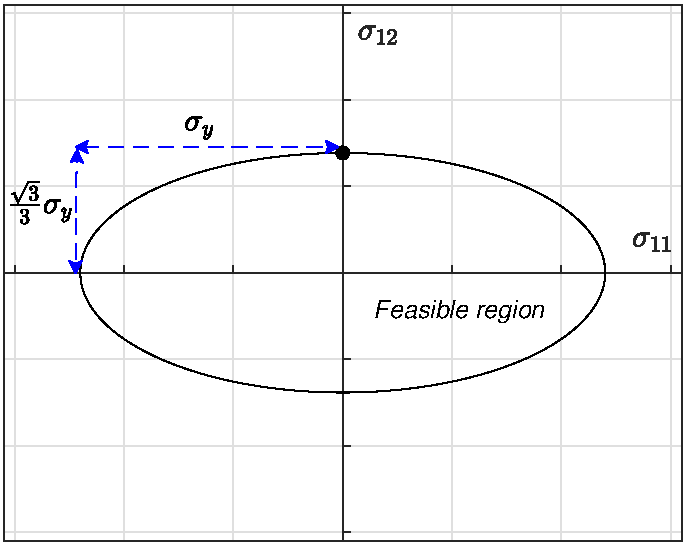
\includegraphics[scale=0.8]{FIG16_YIELDLOCUS}
	\caption{Feasible space and yield locus for the $J_2$ model. At the 
	boundary of the ellipse,
		$\sqrt{3J_2}=q$.}
	\label{fig:FIG16_YIELDLOCUS}
\end{figure}

When kinematic
hardening is included, we introduce the effective stress tensor and its
deviatoric part in order to facilitate notational simplicity:
\begin{equation}
	\bm{\zeta} = \bm{\sigma}-\bm{\alpha},\qquad \bm{\zeta}^d =
	\bm{\sigma}^d-\bm{\alpha}^d
	\label{eq:EFFECTIVE_STRESS}
\end{equation}

We now define the following vectors associated with the active tensor
components that explicitly enter subsequent derivations:
\begin{gather}
	\bvec{\alpha}_f = \begin{bmatrix} \alpha_{11} \\ \alpha_{12} 
	\end{bmatrix},\quad
	\bvec{\alpha}^d_f = \begin{bmatrix} \alpha_{11}^d \\ \alpha_{12}^d 
	\end{bmatrix},\quad
	\bvec{\epsilon}^{pl}_f = \begin{bmatrix} \epsilon^{pl}_{11} \\ 
		\gamma^{pl}_{12} \end{bmatrix},\nonumber\\
	\hspace{-0.4cm}\bvec{\sigma}^d_f = \begin{bmatrix} \sigma^d_{11} \\ 
	\sigma^d_{12}
	\end{bmatrix},\quad\hspace{0.15cm}
	\bvec{\zeta}_f = \begin{bmatrix}
		\zeta_{11} \\ \zeta_{12}
	\end{bmatrix},\quad\hspace{0.15cm}
	\bvec{\zeta}_f^d = \begin{bmatrix}
		\zeta_{11}^d \\ \zeta_{12}^d
	\end{bmatrix}\nonumber
%	\label{eq:FIBER_J2_VECTORS}
\end{gather}
The vector representation of (\ref{eq:J2}) in terms of the effective stress is:
\begin{equation}
	J_2 = \frac{1}{2}(\bvec{\zeta}^d)^T\bmat{J}\bvec{\zeta}^d 
	\label{eq:VECTOR_J2_3D}
\end{equation}
\noindent where matrix $\bmat{J} = \text{diag}[1, 1, 1, 2,2,2]$ is introduced to
account for the symmetry of $\bm{\zeta}^d$.

We now seek a mapping from the deviatoric stress space onto the fiber stress 
space $S$ of the deviatoric
effective stress vector $\bvec{\zeta}^d$ that preserves the inner product and, 
thus, the second deviatoric invariant $J_2$. The non-zero components of 
$\bvec{\zeta}^d$ are $\zeta_{11}^d,\ \zeta_{22}^d,\ \zeta_{33}^d,\
\zeta_{12}^d,\ \zeta_{21}^d$ and thus we can establish the following mappings
between the active components of $\bvec{\zeta}^d$ and $\bvec{\zeta}_f$:
\begin{equation}
	\bvec{\zeta}^d = \bmat{Q}\bvec{\zeta}_f,\qquad \bvec{\zeta}^d_f =
	\bmat{S}\bvec{\zeta}_f
	\label{eq:MAPPING}
\end{equation}
where the mapping matrices above are given by:
\begin{equation}
	\bmat{Q} = \begin{bmatrix}
		\frac{2}{3} & -\frac{1}{3} & -\frac{1}{3} & 0 & 0 & 0 \\
		0 & 0 & 0 & 1 & 0 & 0
	\end{bmatrix}^T,\qquad \bmat{S} = \begin{bmatrix}
		\frac{2}{3} & 0\\
		0 & 1
	\end{bmatrix}
	\label{eq:MAPPING_MATRIX}
\end{equation}
We can now express $J_2$ purely in terms of $\bvec{\zeta}_f$:
\begin{equation}
	J_2 = \frac{1}{2}(\bvec{\zeta}^d)^T\bmat{J}\bvec{\zeta}^d = 
	\frac{1}{2}\bvec{\zeta}_f^T\bmat{Q}^T\bmat{J}\bmat{Q}\bvec{\zeta}_f =
	\frac{1}{2}\bvec{\zeta}_f^T\bmat{V}\bvec{\zeta}_f = \frac{1}{2}\Vert
	\bvec{\zeta}_f\Vert^2_{\bm{V}}
	\label{eq:J2_EQUIV}
\end{equation}
where $\bmat{V} =\text{diag}[\frac{2}{3}, 2]$ and the notation used for the 
inner product induced by matrix $\bmat{A}$ between vectors 
$\bvec{w},\ \bvec{v}$ is $(\bvec{w},\bvec{v})_{\bm{A}} =
\bvec{w}^T\bmat{A}\bvec{v}$, which leads to the notation adopted in Eq. 
(\ref{eq:J2_EQUIV}).

With these derivations at hand, system (\ref{eq:THREE_D_RATE}) can be recast in
the constrained fiber stress state as follows:
\begin{subequations}
	\begin{alignat}{3}
		&\dot{\bvec{\epsilon}}_f &&= \dot{\bvec{\epsilon}}_f^{el} +
		\dot{\bvec{\epsilon}}_f^{pl}\quad& \text{(Strain
			decomposition)}\label{eq:FIBER_RATE_DECOMP}\\
		&\dot{\bvec{\sigma}}_f &&= \bmat{C}^{el}\left[\dot{\bvec{\epsilon}}_f -
		\dot{\bvec{\epsilon}}_f^{pl} \right]\quad& \text{(Elastic constitutive
			law)}\label{eq:FIBER_CONSTITUTIVE_LAW}\\
		&\dot{\bvec{\epsilon}}_f^{pl} &&= \dot{\lambda}\bvec{n}\quad& 
		\text{(Flow
			rule)}\label{eq:FIBER_FLOW_RULE}\\
		&\dot{\bvec{\alpha}}_f &&= 
		\dot{\lambda}H_{kin}\bmat{V}^{-1}\bvec{n}\quad& \text{(Kinematic
			hardening law)}\label{eq:FIBER_BACK_STRESS}\\
		&\dot{q}_f &&= \dot{\lambda}\frac{\partial q_f}{\partial
			e_f^{pl}}\quad& \text{(Isotropic hardening law)}
		\label{eq:FIBER_CURRENT_YIELD_STRESS}\\
		&\Phi(\bvec{\zeta}_f,e^{pl}) &&=
		\sqrt{\frac{3}{2}}\Vert\bvec{\zeta}_f\Vert_{\bm{V}} - q_f(e_f^{pl}) 
		\leq 0\quad&
		\text{(Yield criterion)}\label{eq:FIBER_J2_YIELD_FUNC} 
	\end{alignat}
	\label{eq:FIBER_RATE_SYSTEM}
\end{subequations}

\noindent Vector $\bvec{n}$ is expressed as follows:
\begin{equation}
	\bvec{n} =  \frac{\partial \Phi}{\partial \bm{\sigma}_f} = 
	- \frac{\partial \Phi}{\partial \bm{\alpha}_f} =
	\sqrt{\frac{3}{2}}\frac{\bmat{V}\bvec{\zeta}_f}{\Vert\bvec{\zeta}_f\Vert_{\bm{V}}}
	\label{eq:VECTOR_n}
\end{equation}
Equations (\ref{eq:CURRENT_YIELD_STRESS}), (\ref{eq:EQUIV_PLASTIC_STRAIN})
remain the same in the current system. In addition, note that for the 
$J_2$ model, the left-hand side of eq. (\ref{eq:BACK_STRESS}) is a deviatoric 
tensor whereas in (\ref{eq:FIBER_BACK_STRESS}) it has been mapped to fiber 
stress space $\mathcal{S}$.


%%%%%%%%%%%%%%%%%%%%  SECTION 3 - SUBSECTION 2 %%%%%%%%%%%%%%%%%%%%%%%%%%%%%%%%
\subsection{Continuous Tangent Modulus}\label{section:CH3-S3SS2}

The continuous elastoplastic modulus $\bmat{C}^{ep}$ is found by enforcing the
plastic consistency condition (\ref{eq:PLASTIC_CONSISTENCY_CONDITION}) during a 
plastic step:
\begin{equation}
	\bvec{n}^T\dot{\bvec{\zeta}}_f-\dot{\lambda}\frac{\partial q_f}{\partial
		e_f^{pl}} = 0
	\label{eq:FIBER_PLASTIC_CONSISTENCY_ENF}
\end{equation}
The rate form for the effective stress is given by combining Eqs.
(\ref{eq:FIBER_CONSTITUTIVE_LAW}), (\ref{eq:FIBER_BACK_STRESS}) with
$\dot{\bvec{\zeta}}_f = \dot{\bvec{\sigma}}_f - \dot{\bvec{\alpha}}_f$:
\begin{equation}
	\dot{\bvec{\zeta}}_f = \bmat{C}^{el}\dot{\epsilon}_f -
	\dot{\lambda}\bmat{Z}\bvec{n}
	\label{eq:RATE_FORM_EFFECTIVE}
\end{equation}
\noindent where $\bmat{Z} = \bmat{C}^{el}+H_{kin}\bmat{V}^{-1}$.
Substituting (\ref{eq:RATE_FORM_EFFECTIVE}) into
(\ref{eq:FIBER_PLASTIC_CONSISTENCY_ENF}) and solving for $\dot{\lambda}$ we get:
\begin{equation}
	\dot{\lambda} =
	\frac{\bvec{n}^T\bmat{C}^{el}\dot{\bvec{\epsilon}}_f}{\bvec{n}^T\bmat{Z}\bvec{n}+
		\frac{\partial q_f}{\partial e_f^{pl}}}
	\label{eq:PLASTIC_PARAM_RATE}
\end{equation}
Finally, by making use of (\ref{eq:PLASTIC_PARAM_RATE}),
(\ref{eq:FIBER_FLOW_RULE}) and (\ref{eq:FIBER_CONSTITUTIVE_LAW}), we arrive at
the expression for the continuous elastoplastic modulus:
\begin{equation}
	\bmat{C}^{pl} =
	\bmat{C}^{el}-\frac{\bvec{m}\bvec{m}^T}{\bvec{n}^T\bmat{Z}\bvec{n}+
		\frac{\partial q_f}{\partial e_f^{pl}}}
	\label{eq:CONT_ELASTOPLASTIC_MODULUS}
\end{equation}
\noindent where $\bvec{m} = \bmat{C}^{el}\bvec{n}$.

%%%%%%%%%%%%%%%%%%%%  SECTION 4 %%%%%%%%%%%%%%%%%%%%%%%%%%%%%%%%
\section{Implicit Integration of Rate Equations}\label{section:CH3-S4}
%%%%%%%%%%%%%%%%%%%%%%%%%%%%%%%%%%%%%%%%%%%%%%%%%%%%%%%%%%%%%%%%

We employ the fully implicit backward Euler method to discretize the rate
constitutive equations in system (\ref{eq:FIBER_RATE_SYSTEM}) in the pseudotime
interval $[t_n,t_{n+1}]$. We regard the incremental/iterative process as strain
driven, in that at the start of increment $n$, the dependent state variables 
for each fiber,
$S_n=\{\bvec{\epsilon}_f,\bvec{\epsilon}_f^{pl},\bvec{\alpha}_f,e_f^{pl}\}_n$, 
are
known and stored. We also know the increment in the centerline strain vector
$\bvec{d}$, $\Delta\bvec{d}$. The incremental strain vector for the current
fiber is then determined using eq. (\ref{eq:f2}):
\begin{equation*}
	\Delta\bvec{\epsilon}_f = \bmat{N}_s\Delta\bvec{q}
	\label{eq:INCREMENTAL_STRAINS}
\end{equation*}
Given the incremental strain vector $\Delta\bvec{\epsilon}_f$, 
we need to update the state variables for $t_{n+1}$:  $S_n\rightarrow S_{n+1}$.
In what follows we ommit the subscript denoting the vector pertains to the fiber
state: 
\begin{equation*}
	S_n \equiv
	\{\bvec{\epsilon}_n,\bvec{\epsilon}_n^{pl},\bvec{\alpha}_n,e_n^{pl}\},\qquad
	S_{n+1} \equiv
	\{\bvec{\epsilon}_{n+1},\bvec{\epsilon}_{n+1}^{pl},\bvec{\alpha}_{n+1},e_{n+1}^{pl}\},
\end{equation*}

The update of the fiber total strain vector $\bvec{\epsilon}$ is trivial:
$\bvec{\epsilon}_{n+1} = \bvec{\epsilon}_n + \Delta\bvec{\epsilon}$. For the
remaining state variables the rate system (\ref{eq:FIBER_RATE_SYSTEM}) is 
discretized as follows:
\begin{subequations}
	\begin{alignat}{2}
		&\bvec{\sigma}_{n+1} &&=  
		\bmat{C}^{el}\left[\bvec{\epsilon}_{n+1} -
		\bvec{\epsilon}_{n+1}^{pl} 
		\right]\label{eq:FIBER_CONSTITUTIVE_LAW_DISCR}\\
		&\bvec{\epsilon}_{n+1}^{pl} &&= \bvec{\epsilon}_{n}^{pl} +
		\dot{\lambda}\bvec{n}_{n+1}
		\label{eq:FIBER_FLOW_RULE_DISCR}\\
		&\bvec{\alpha}_{n+1} &&=\bvec{\alpha}_{n} + 
		\lambda H_{kin}\bmat{V}^{-1}\bvec{n}_{n+1}
		\label{eq:FIBER_BACK_STRESS_DISCR}\\
		&q_{n+1} &&= q_{n} + \lambda\frac{\partial q_{n+1}}{\partial
			e_{n+1}^{pl}}\label{eq:FIBER_CURRENT_YIELD_STRESS_DISCR}\\
		&\Phi(\bvec{\zeta}_{n+1},e_{n+1}^{pl}) &&=
		\sqrt{\frac{3}{2}}\Vert\bvec{\zeta}_{n+1}\Vert_{\bm{V}} -
		q_{n+1}(e_{n+1}^{pl}) \leq 0
		\label{eq:FIBER_J2_YIELD_FUNC_DISCR}
	\end{alignat}
	\label{eq:FIBER_DISCR_SYSTEM}
\end{subequations}
\noindent and
\begin{equation}
	\bvec{\zeta}_{n+1} = \bvec{\sigma}_{n+1} - \bvec{\alpha}_{n+1}
	\label{eq:DISCR_EFFECTIVE}
\end{equation}


%%%%%%%%%%%%%%%%%%%%  SECTION 4 - SUBSECTION 1 %%%%%%%%%%%%%%%%%%%%%%%%%%%%%%%%
\subsection{Elastic Predictor - Plastic Corrector 
algorithm}\label{section:CH3-S4SS1}

It is convenient to recast system (\ref{eq:FIBER_DISCR_SYSTEM})
purely in terms of stress by utilizing
(\ref{eq:DISCR_EFFECTIVE}),(\ref{eq:FIBER_CONSTITUTIVE_LAW_DISCR}),(\ref{eq:FIBER_BACK_STRESS_DISCR}):

\hspace{-0.3cm}\begin{minipage}{0.4\linewidth}
	\hspace{1.7cm}\begin{tabular}[]{c}
		\textbf{Stress rate system}\\
		\specialrule{2.pt}{1pt}{-15pt}
	\end{tabular}
	\begin{subequations}
		\begin{align}
			\dot{\bvec{\zeta}} &=
			\bmat{C}^{el}\dot{\bvec{\epsilon}}-\dot{\lambda}\bmat{Z}\bvec{n}\label{eq:EFF_RATE1}\\
			\dot{q} &= \dot{\lambda}\frac{\partial q}{\partial
				e^{pl}}\label{YIELD_RATE2}
		\end{align}
		\label{eq:REDUCED_RATE_SYS}
	\end{subequations}
\end{minipage}
\begin{minipage}{0.55\linewidth}
	\hspace{1.7cm}\begin{tabular}[]{c}
		\textbf{Discretized system}\\
		\specialrule{1.5pt}{2.5pt}{-15pt}
	\end{tabular}
	\begin{subequations}
		\begin{align}
			\bvec{\zeta}_{n+1} &= \bvec{\zeta}_n +
			\bmat{C}^{el}\Delta\bvec{\epsilon}_{n+1}-\lambda\bmat{Z}\bvec{n}_{n+1}
			\label{eq:EFF_DISCR1}\\
			q_{n+1} &= q_n + \lambda\frac{\partial q_{n+1}}{\partial
				e_{n+1}^{pl}}\label{eq:YIELD_DISCR2}
		\end{align}
		\label{eq:REDUCED_DISCR_SYS}
	\end{subequations}
\end{minipage}

We need not differentiate between initial and final value for the plastic
parameter $\lambda$ since it is initialized to zero at the beginning of every
step: $\lambda_n = 0$. The solution of (\ref{eq:REDUCED_DISCR_SYS}) is based on
a two-step procedure. The first phase is called trial elastic step, where 
we assume that the increment $\Delta\bvec{\epsilon}$ is elastic and all state 
variables are updated by setting $\lambda=0$: $S_n\rightarrow S_{n+1}^{TR}$. If 
the trial stresses satisfy the yield condition $\Phi^{TR}_{n+1} < 0$, then the 
step
was indeed elastic and we can set $S^{TR}_{n+1}\rightarrow S_{n+1}$. If the 
yield 
criterion is violated, $\Phi^{TR}_{n+1}>0$, then the step is plastic and we 
need to 
apply (plastic) corrections to the state variables so that, upon convergence, 
we have achieved $\Phi_{n+1} = 0$. This procedure is referred to as
Elastic Predictor - Plastic Corrector algorithm and can be traced back to the
work of Wilkins\cite{Wilkins1963}. It has enjoyed widespread
application in solving problems in
elastoplasticity\cite{Dodds1987,DeAngelis2015,Clausen2006,Hopperstad1995,Scherzinger2017,Hartloper2021}
and the basic relations for each step are summarized below.

\hspace{-1.2cm}\begin{minipage}{0.5\linewidth}
	\hspace{1cm}\begin{tabular}[]{c}
		\textbf{Elastic Predictor}\\
		\specialrule{2.pt}{1pt}{-15pt}
	\end{tabular}
	\begin{subequations}
		\begin{align}
			\bvec{\zeta}_{n+1}^{TR} &= \bmat{C}^{el}\left[\bvec{\epsilon}_{n+1}-
			\bvec{\epsilon}_n^{pl}\right]-\bvec{\alpha}_n\label{eq:TRIAL_EFFECTIVE}\\
			q_{n+1}^{TR} &= q_n \label{eq:TRIAL_YIELD}\\
			\Phi_{n+1}^{TR} &=
			f_(\bvec{\zeta}_{n+1}^{TR},q_{n+1}^{TR})\label{eq:TRIAL_YIELDFUN}
		\end{align}
		\label{eq:ELASTIC PREDICTOR}
	\end{subequations}
\end{minipage}
\hspace{0.3cm}\begin{minipage}{0.05\linewidth}
	$\xrightarrow{\Phi_{n+1}^{TR}>0}$
\end{minipage}
\hspace{0.70cm}\begin{minipage}{0.4\linewidth}
	\hspace{1.7cm}\begin{tabular}[]{c}
		\textbf{Plastic Corrector}\\
		\specialrule{2.pt}{1pt}{-15pt}
	\end{tabular}
	\begin{subequations}
		\begin{align}
			\bvec{\zeta}_{n+1} &= \bvec{\zeta}_{n+1}^{TR} - 
			\lambda\bmat{Z}\bvec{n}_{n+1}\label{eq:CORRECTOR_EFFECTIVE}\\
			q_{n+1} &= q_{n+1}^{TR} + \lambda\frac{\partial q_{n+1}}{\partial
				e_{n+1}^{pl}}\label{eq:CORRECTOR_YIELD}\\
			\Phi_{n+1} &= 0\label{eq:CORRECTOR_YIELDFUN}
		\end{align}
		\label{eq:PLASTIC CORRECTOR}
	\end{subequations}
	\label{eq:PLASTIC_CORRECTOR_SYS}
\end{minipage}

The Plastic Corrector step is a system of 4 nonlinear algebraic equations with 
4 unknowns, $\{\zeta_{11,n+1}, \zeta_{12,n+1}, q_{n+1}, \lambda\}$, and
generally a local Newton method is required to determined the unknowns. It
should be stressed here that, in multiaxial constitutive algorithms that do not
make use of the mapping as developed here, this local process is nested within 
an upper level Newton procedure that enforces the zero transverse
stress condition.

Substituting Eqs. (\ref{eq:CORRECTOR_EFFECTIVE}),(\ref{eq:CORRECTOR_YIELD})
into (\ref{eq:CORRECTOR_YIELDFUN}) furnishes a nonlinear scalar equation that
needs to be solved for $\lambda$. Once $\lambda$ is computed, then the fiber
state can be updated $S_{n+1}^{TR}\rightarrow S_{n+1}$. Refer also to
Box ~\ref{Box:BOX1} for a detailed summary of the plastic updates. Detailed
expressions for the local Newton method on $\Phi_{n+1}(\lambda)=0$ are provided 
in Appendix \ref{appendix:APPENDIX_C}.

%%%%%%%%%%%%%%%%%%%%  SECTION 4 - SUBSECTION 2 %%%%%%%%%%%%%%%%%%%%%%%%%%%%%%%%
\subsection{Consistent Tangent Modulus}\label{section:CH3-S4SS2}

The tangent modulus consistent with the numerical discretization used on system
(\ref{eq:FIBER_RATE_SYSTEM}) is necessary to restore the quadratic rates of
convergence for the global Newton method\cite{Simo1985}. That is:
\begin{equation}
	\bmat{C}_c^{pl} =
	\frac{\text{d}\bvec{\sigma}_{n+1}}{\text{d}\bvec{\epsilon}_{n+1}}
	\label{eq:CONSISTENT_TANG_FORM}
\end{equation}
We take the differentials of (\ref{eq:FIBER_CONSTITUTIVE_LAW_DISCR}),
(\ref{eq:FIBER_BACK_STRESS_DISCR}) and (\ref{eq:FIBER_J2_YIELD_FUNC_DISCR}), 
using the fact that 
$\text{d}\bvec{\zeta}_{n+1} = \text{d}\bvec{\sigma}_{n+1} -
\text{d}\bvec{\alpha}_{n+1}$ from (\ref{eq:DISCR_EFFECTIVE}) and arrive at the
following system:
\begin{subequations}
	\begin{equation}
		\begin{bmatrix}
			\bmat{C}^{el}+\lambda\bmat{\Psi}_{n+1} & 
			-\lambda\bmat{\Psi}_{n+1}\\
			-\lambda\bmat{\Psi}_{n+1} & 
			H_{kin}^{-1}\bmat{V}+\lambda\bmat{\Psi}_{n+1}
		\end{bmatrix}\begin{bmatrix}
			\text{d}\bvec{\sigma}_{n+1}\\
			\text{d}\bvec{\alpha}_{n+1}
		\end{bmatrix} = \begin{bmatrix}
			\text{d}\bvec{\epsilon}_{n+1}-\text{d}\lambda\bvec{n}_{n+1}\\
			\text{d}\lambda\bvec{n}_{n+1}
		\end{bmatrix}
		\label{eq:DIFF_SYSTEM}
	\end{equation}
	\begin{equation}
		\bvec{n}_{n+1}^T\left[\text{d}\bvec{\sigma}_{n+1} -
		\text{d}\bvec{\alpha}_{n+1}\right] = \text{d}\lambda
		\frac{\partial q_{n+1}}{\partial e_{n+1}^{pl}}
		\label{eq:YIELD_FUNC_DIFF}
	\end{equation}
	\label{eq:DIFF_SYS_YIELD}
\end{subequations}

\noindent where $\bmat{\Psi}$ is given as follows:
\begin{equation}
	\bmat{\Psi} = \frac{\partial\bvec{n}}{\partial \bvec{\zeta}}=
	\frac{\partial^2 f}{\partial \bvec{\zeta}^2} = \frac{1}{\Vert
		\bvec{\zeta}\Vert_{\bm{V}}}\left[ \bmat{V}-\bvec{n}\bvec{n}^T\right]
	\label{eq:B}
\end{equation}
Upon solving (\ref{eq:DIFF_SYSTEM}) for $\text{d}\bvec{\sigma}_{n+1}$,
$\text{d}\bvec{\alpha}_{n+1}$ we substitute them into (\ref{eq:YIELD_FUNC_DIFF})
and solve for d$\lambda$:
\begin{equation}
	\text{d}\lambda =
	\frac{\bvec{n}_{n+1}^T\left[\bmat{\Xi}_{11}+\bmat{\Xi}_{12}^T\right]\text{d}\bvec{\epsilon}_{n+1}}{\bvec{n}_{n+1}^T\bmat{T}\bvec{n}_{n+1}+
		\frac{\partial q_{n+1}}{\partial e_{n+1}^{pl}}}
	\label{eq:DE_GAMMA}
\end{equation}
Finally, substituting d$\lambda$ into (\ref{eq:FIBER_CONSTITUTIVE_LAW_DISCR}) 
furnishes the formula for the consistent tangent modulus:
\begin{equation}
	\bmat{C}_c^{pl} = 
	\bmat{\Xi}_{11}-\frac{\bvec{N}_{n+1}\bvec{N}_{n+1}^T}{1+\delta_{n+1}}
	\label{eq:CONSISTENT TANGENT MOD}
\end{equation}
Details regarding all newly defined vectors and matrices involved in the
derivation of $\bmat{C}_c^{pl}$ is given in Appendix \ref{appendix:APPENDIX_D}. 
In Box ~\ref{Box:BOX1} 
we have summarised the return mapping algorithnm for a fiber.

%%%%%%%%%%%%%%%%%%%%  SECTION 4 - SUBSECTION 3 %%%%%%%%%%%%%%%%%%%%%%%%%%%%%%%%
\subsection{Consistent Section Stiffness}\label{section:CH3-S4SS3}

Once the stress update on a particular fiber has been carried out, its
contribution to the stress resultant vector and the section stiffness are
accounted for via a midpoint integration rule along the section height (see Eqs.
(\ref{eq:STRESS_RES_CONJUGATE}), (\ref{eq:FIB_STIFF_CONTRIB}).

% ~~~~~~~~~~~~~~~~~~~~~~ BOX 1  ~~~~~~~~~~~~~~~~~~~~~``
{
	\centering
	\begin{tcolorbox}[tikznode boxed title,enhanced,arc=0mm,interior
		style={white}, colbacktitle=white,coltitle=black,
		width=5in,top=5pt,bottom=10pt,boxrule=1pt,toprule=1pt,fonttitle=\bfseries,title={Box
		 1
			: Summary of Elastic Predictor - Plastic Corrector 
			algorithm.},sharp corners,
		boxed title style = {size=normal,colframe=white,boxrule=0pt}]
		$\bullet\hspace{0.5cm}$  \textbf{Start of step - Elastic Predictor}
		
		\vspace{-1.2cm}
		\begin{minipage}[t]{0.6\linewidth}
			\begin{alignat*}{2}
				\blacksquare\hspace{0.3cm}	&\bvec{\epsilon}^{pl,TR}_{n+1} &&= 
				\bvec{\epsilon}^{pl}_n\\
				\blacksquare\hspace{0.3cm}	&\bvec{\sigma}^{TR}_{n+1} &&=
				\bmat{C}^{el}\left[\bvec{\epsilon}_{n+1}-\bvec{\epsilon}^{pl}_n\right]\\
				\blacksquare\hspace{0.3cm}	&\bvec{\alpha}^{TR}_{n+1} &&= 
				\bvec{\alpha}_n\\
			\end{alignat*}
		\end{minipage}
		\begin{minipage}[t]{0.22\linewidth}
			\begin{alignat*}{2}
				\blacksquare\hspace{0.3cm} &e^{pl,TR}_{n+1} &&= e^{pl}_n\\
				\blacksquare\hspace{0.3cm}	&q^{TR}_{n+1} &&= q_n\\
				\blacksquare\hspace{0.3cm}	&f_{n+1}^{TR} &&=
				\Phi(\bvec{\zeta}_{n+1}^{TR},q_{n+1}^{TR})
			\end{alignat*}
		\end{minipage}
		
		\vspace{-0.3cm}
		$\bullet\hspace{0.5cm}\text{IF}\ \Phi_{n+1}^{TR}<0\rightarrow$  
		\textbf{Elastic Step}
		
		\vspace{-1.2cm}
		\hspace{-1.03cm}\begin{minipage}[t]{0.6\linewidth}
			\begin{alignat*}{2}
				\blacksquare\hspace{0.3cm}	&\bvec{\epsilon}^{pl}_{n+1} &&=
				\bvec{\epsilon}^{pl,TR}_{n+1}\\
				\blacksquare\hspace{0.3cm}	&\bvec{\sigma}_{n+1}
				&&=\bvec{\sigma}^{TR}_{n+1}\\
				\blacksquare\hspace{0.3cm}	&\bvec{\alpha}_{n+1} &&= 
				\bvec{\alpha}^{TR}_{n+1}
			\end{alignat*}
		\end{minipage}
		\begin{minipage}[t]{0.41\linewidth}
			\begin{alignat*}{2}
				\blacksquare\hspace{0.3cm} &e^{pl}_{n+1} &&= e^{pl,TR}_{n+1}\\
				\blacksquare\hspace{0.3cm}	&q_{n+1} &&= q^{TR}_{n+1}\\
				\blacksquare\hspace{0.3cm}	&\bmat{C} &&= \bmat{C}^{el}
			\end{alignat*}
		\end{minipage}
		
		\vspace{0.6cm}
		$\bullet\hspace{0.5cm}\text{ELSE}\ f_{n+1}^{TR}>0\rightarrow$  
		\textbf{Plastic Corrector}
		\begin{enumerate}
			\item Iteratively solve (\ref{eq:PLASTIC_CORRECTOR_SYS}) for 
			$\lambda$:
			$\lambda^{j+1}=\lambda^j-\frac{\Phi_{n+1}^j}{(\frac{\text{d}\Phi_{n+1}}{\text{d}\lambda})^j}$,
			with $\lambda^0 = 0$, $\Phi_{n+1}^0 = \Phi_{n+1}^{TR}$. Loop 
			termination:
			$|\Phi_{n+1}^{j+1}|\leq e_{tol}$, where $e_{tol}$ small.
			\item Update state variables:
			
			\vspace{-1.7cm}
			\hspace{-0.15cm}\begin{minipage}[t]{0.3\linewidth}
				\begin{alignat*}{2}
					\blacksquare\hspace{0.3cm}	&\bvec{\zeta}_{n+1} &&=
					\bm{\Omega}(\lambda)\bvec{\zeta}_{n+1}^{TR}\\
					\blacksquare\hspace{0.3cm}	&\bvec{\epsilon}^{pl}_{n+1} &&= 
					\bvec{\epsilon}^{pl}_n + \lambda\bvec{n}_{n+1}\\
					\blacksquare\hspace{0.3cm}	&\bvec{\alpha}_{n+1} &&= 
					\bvec{\alpha}_n + \lambda 
					H_{kin}\bmat{V}^{-1}\bvec{n}_{n+1}\\
				\end{alignat*}
			\end{minipage}
			\begin{minipage}[t]{0.4\linewidth}
				\begin{alignat*}{2}
					\blacksquare\hspace{0.3cm} &\bvec{\sigma}_{n+1} &&= 
					\bvec{\zeta}_{n+1} + \bvec{\alpha}_{n+1}\\
					\blacksquare\hspace{0.3cm} &e^{pl}_{n+1} &&= e^{pl}_n + 
					\lambda \\
					\blacksquare\hspace{0.3cm}	&q_{n+1} &&= q_n + 
					\lambda\frac{\partial
						q_{n+1}}{\partial e_{n+1}^{pl}}
				\end{alignat*}
			\end{minipage}
			
			\vspace{-0.5cm}
			\item Get consistent tangent modulus
			\vspace{-0.5cm}
			$$\bmat{C}=\bmat{C}_c^{pl} = 
			\bmat{\Xi}_{11}-\frac{\bvec{N}_{n+1}\bvec{N}_{n+1}^T}{1+\delta_{n+1}}$$
		\end{enumerate}
		See Appendix \ref{appendix:APPENDIX_C} for $\bm{\Omega}(\lambda)$.
		\step\label{Box:BOX1}
	\end{tcolorbox}
}
\clearpage

Notice that while in the present formulation $C_{21}=C_{12}$, this will not be
the case if a generalized integration rule is used for the rate equations. In
such a scenario, if enforcement of the plastic consistency does not correspond
to the interior time $t_a\in[t_n, t_{n+1}]$ chosen, that is $\Phi_a=0$, then 
the consistenttangent will not be symmetric. For more details on this refer to
\cite{Ortiz1985}.

%%%%%%%%%%%%%%%%%%%%  SECTION 5 %%%%%%%%%%%%%%%%%%%%%%%%%%%%%%%%
\section{Numerical Examples}\label{section:CH3-S5}
%%%%%%%%%%%%%%%%%%%%%%%%%%%%%%%%%%%%%%%%%%%%%%%%%%%%%%%%%%%%%%%%

%%%%%%%%%%%%%%%%%%%%  EXAMPLE 1 %%%%%%%%%%%%%%%%%%%%%%%%%%%%%%%%
\subsection{Accuracy of the Proposed Algorithm}    % EXAMPLE 1

Iso-error maps are commonly used to test the accuracy of return-mapping 
algorithms in elastoplasticity\cite{DeSouza2011}. The contours are generated by 
imposing a family of stress or strain prescribed loadings from a selected point 
on the yield surface which cause further plastification (no unloading). For 
each load incrementation, the error is computed as the relative difference 
between the stress predicted by the proposed algorithm and ``exact"" stress. 
The exact stress is typically found by imposing the same increment in a number 
of sequencial subincrements, $n_s$. A convergence analysis is required to 
ensure that subincrementation indeed converges to a stress point. In the 
present study it was found that for $n_s\geq 500$ the stress components had 
achieved convergence with respect to the first 7 decimal points. Therefore, we 
use $n_s = 500$. The error plotted is given by:
\begin{equation}
	err = \frac{\Vert 
		\bvec{\sigma}^*-\bvec{\sigma}\Vert}{\Vert\bvec{\sigma}^*\Vert}\cdot 100
	\label{eq:ERROR}
\end{equation}
\noindent where $\bvec{\sigma}^*$ is the exact stress vector and 
$\bvec{\sigma}$ the one predicted by the proposed scheme by solving in one 
step. The three points on the yield surface that are selected and shown
in Fig. \ref{fig:FIG17_ISO_MAP_SCENARIOS} correspond to an initial state of 
pure shear (A), mixed 
state where $\sigma_{11,0}=\sigma_{12,0}$ (B) and a pure uniaxial stress state 
(C). 
For each of these initial states the family of strain increments are imposed 
along the directions shown, with range up to 
$\Delta\Vert\bvec{\epsilon}\Vert=5\epsilon_y$, where $\epsilon_y$ is the yield 
strain in tension/compression. The material data used are: $E=2.1\times 10^5,\ 
\sigma_y = 2.4\times 10^2$ and Poisson's ratio $\nu=0.3$. For the hardening 
cases, linear isotropic and 
kinematic moduli were prescribed as follows: $H_{iso}=H_{kin} = 10^4$.

\begin{figure}[t]
	\centering
	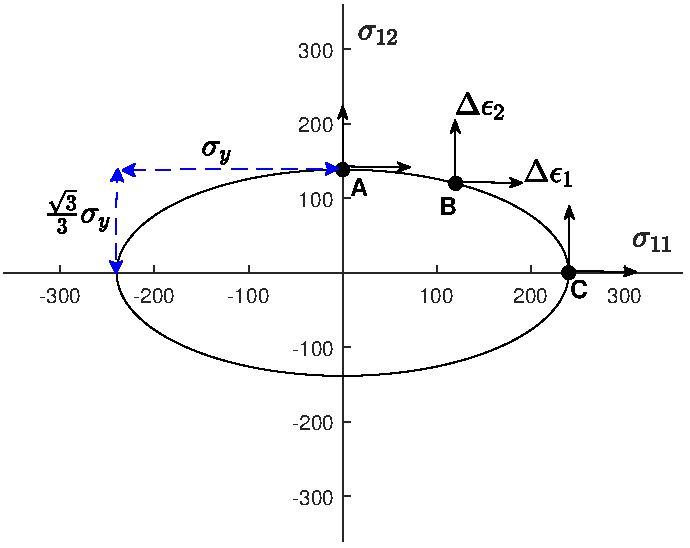
\includegraphics[scale=0.8]{FIG17_SCENARIOS}
	\caption{Points of interest on yield surface and direction of load 
		increments.}
	\label{fig:FIG17_ISO_MAP_SCENARIOS}
\end{figure}

The parameters associated with the horizontal and vertical axes, $a_1,\ a_2$, 
are defined in the following way: $a_1=\Delta\bvec{\epsilon}_1^{}/\epsilon_y$, 
$a_2=\Delta\bvec{\epsilon}_2^{}/\epsilon_y$. As  can be seen from figures 
\ref{fig:FIG18_ISO_MAPS_PERF_PLAST}, \ref{fig:FIG19_ISO_MAPS_HARD}, the 
relative error 
remains small even for quite large increments in the strain vector. Note also 
that for along the semi-major and semi-minor axes in the cases of pure uniaxial 
state and pure shear respectively, the return mapping gives the exact stress 
even without subincrementation. The same is true for point B when the strain 
increments are along a direction around $68^{\circ}$ with respect to $a_1$ axis.

\begin{figure}[b]
	
	\subfloat[Point A]{%
		\hspace{-0.2cm}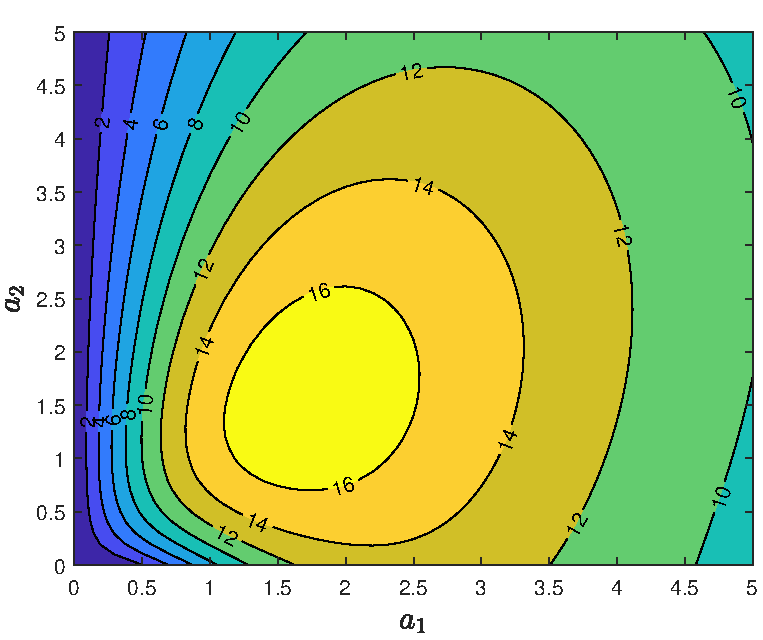
\includegraphics[width=0.33\textwidth]{FIG18_A_ISOMAP_PERF_PLAST}%
		\label{fig:FIG18_A_ISOMAP_PERF_PLAST}%
	}
	\subfloat[Point B]{%
		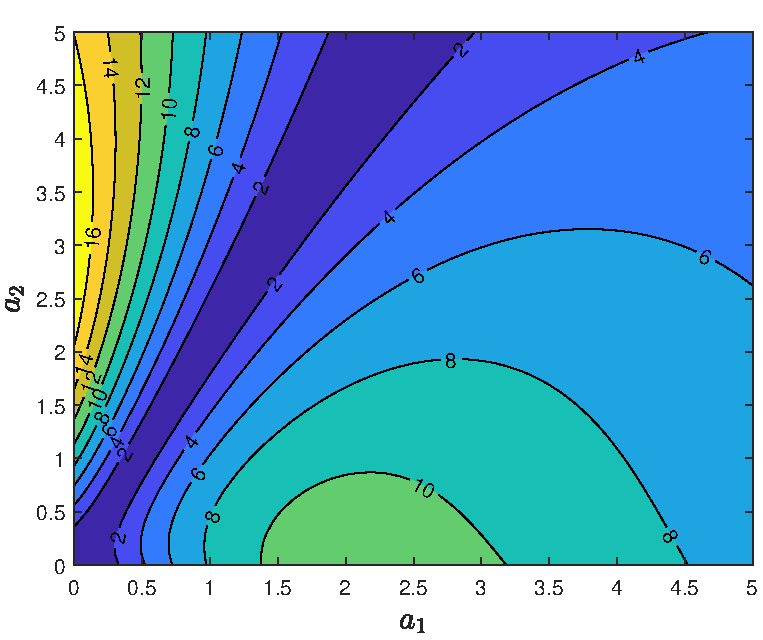
\includegraphics[width=0.33\textwidth]{FIG18_B_ISOMAP_PERF_PLAST}%
		\label{fig:FIG18_B_ISOMAP_PERF_PLAST}%
	}
	\subfloat[Point C]{%
		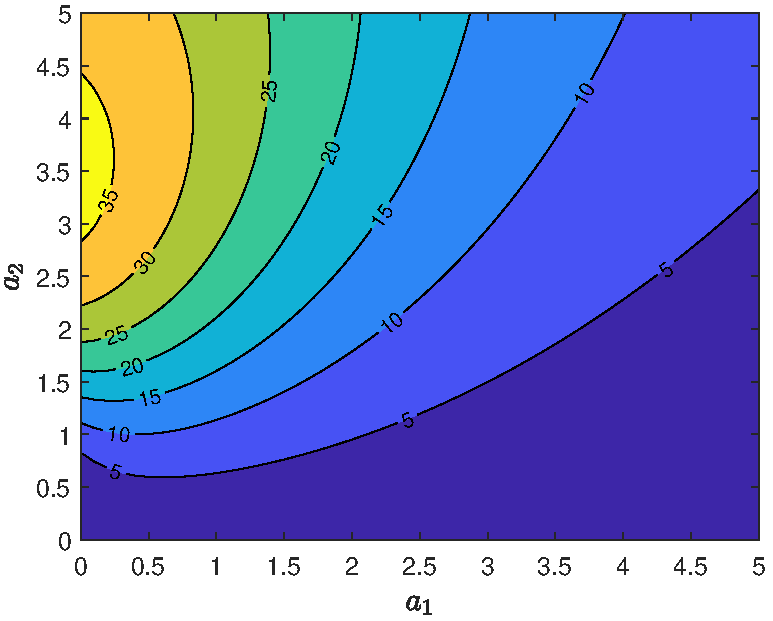
\includegraphics[width=0.33\textwidth]{FIG18_C_ISOMAP_PERF_PLAST}%
		\label{fig:FIG18_C_ISOMAP_PERF_PLAST}%
	}
	\caption{Iso-error maps for a perfectly plastic material.}
	\label{fig:FIG18_ISO_MAPS_PERF_PLAST}
\end{figure} 

\begin{figure}[t]
	
	\subfloat[Point A]{%
		\hspace{-0.2cm}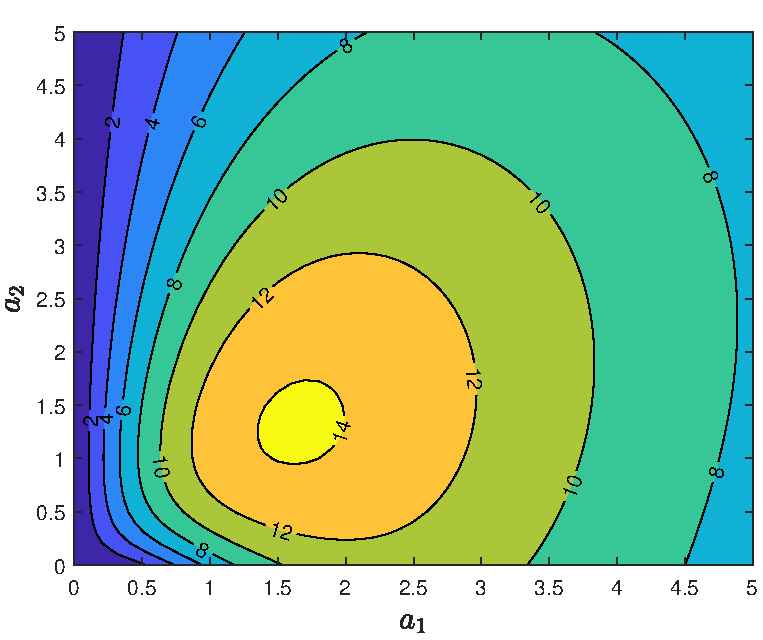
\includegraphics[width=0.33\textwidth]{FIG19_A_ISOMAP_HARD}%
		\label{fig:FIG19_A_ISOMAP_HARD}%
	}
	\subfloat[Point B]{%
		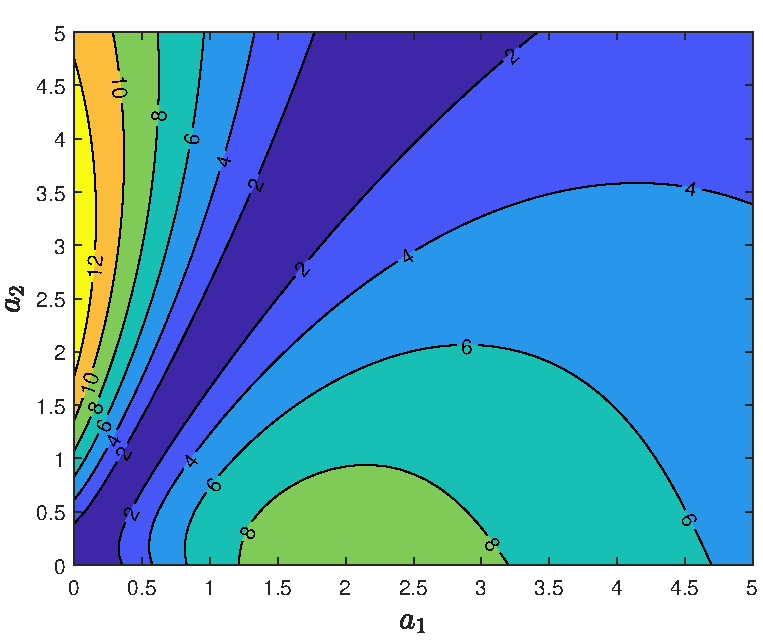
\includegraphics[width=0.33\textwidth]{FIG19_B_ISOMAP_HARD}%
		\label{fig:FIG19_B_ISOMAP_HARDT}%
	}
	\subfloat[Point C]{%
		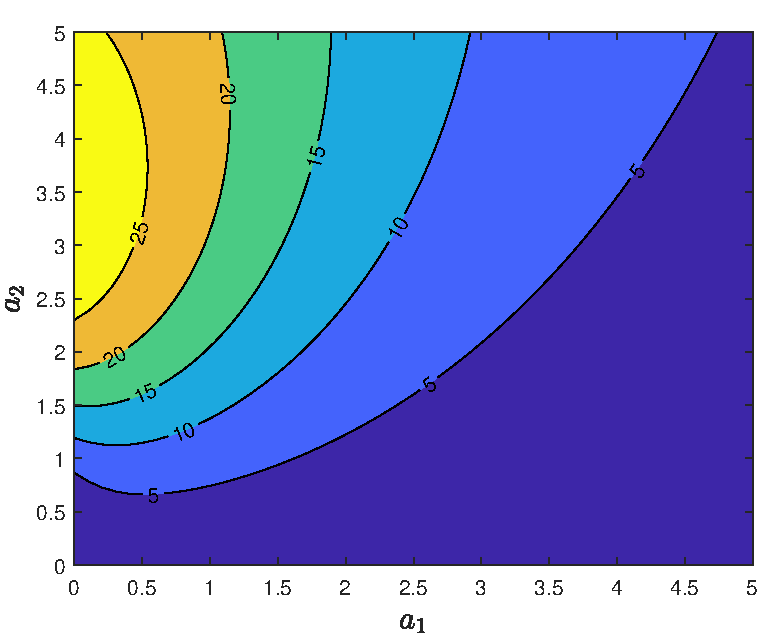
\includegraphics[width=0.33\textwidth]{FIG19_C_ISOMAP_HARD}%
		\label{fig:FIG19_C_ISOMAP_HARD}%
	}
	\caption{Iso-error maps for combined linear isotropic and kinematic 
		hardening.}
	\label{fig:FIG19_ISO_MAPS_HARD}
\end{figure} 

%%%%%%%%%%%%%%%%%%%%  EXAMPLE 2 %%%%%%%%%%%%%%%%%%%%%%%%%%%%%%%%
\subsection{Performance Against Non-Monotonic Strain Histories}

In this benchmark we investigate the performance of the proposed algorithm 
against the three dimensional/axisymmetric procedure typically implemented in 
beam elements when shear-flexure interaction is taken into account using a 
multiaxial law at the fiber level. We also compare it with the plane stress 
projection 
algorithm by Simo\cite{Simo1985}, which we followed in our derivations. In the 
former approach, the return mapping using an implicit integration results in 
the so-called radial return, which doesn't require iterations in the case of 
$J_2$ with perfect plasticity or linear hardening\cite{Wilkins1963}. In 
constrast, the latter requires iterations since the topology of the stress 
space is not as simple as the von Mises cylinder anymore. We show below the 
drastic performance boost when 
using the present algorithm. As already state earlier, this is mainly due to 
the fact that we avoid an additional Newton procedure to enforce the zero 
transverse stress condition. The results for each scenario are shown in the 
tables below. A perfectly plastic material was assumed and both the average 
execution time $t$(sec) and the total number of iterations, $N_i$ are 
considered as performance metrics. The \textit{additional} iterations during 
purely elastic steps are also included in parentheses for the 3D and Simo's 
plane stress algorithm.  Moreover, for each scenario, four 
different incrementations of the strain history are employed, shown in Fig. 
\ref{fig:FIG20_STRAIN_HISTORIES}, and the effect of 
this scaling on the performance is highlighted. Parameter $a$ determines the 
increment ``length'': $\alpha = 
\Vert\Delta\bvec{\epsilon}\Vert^{}/\epsilon_y$. Material data are the same as 
in the previous example. 

\begin{figure}[t]
	\centering
	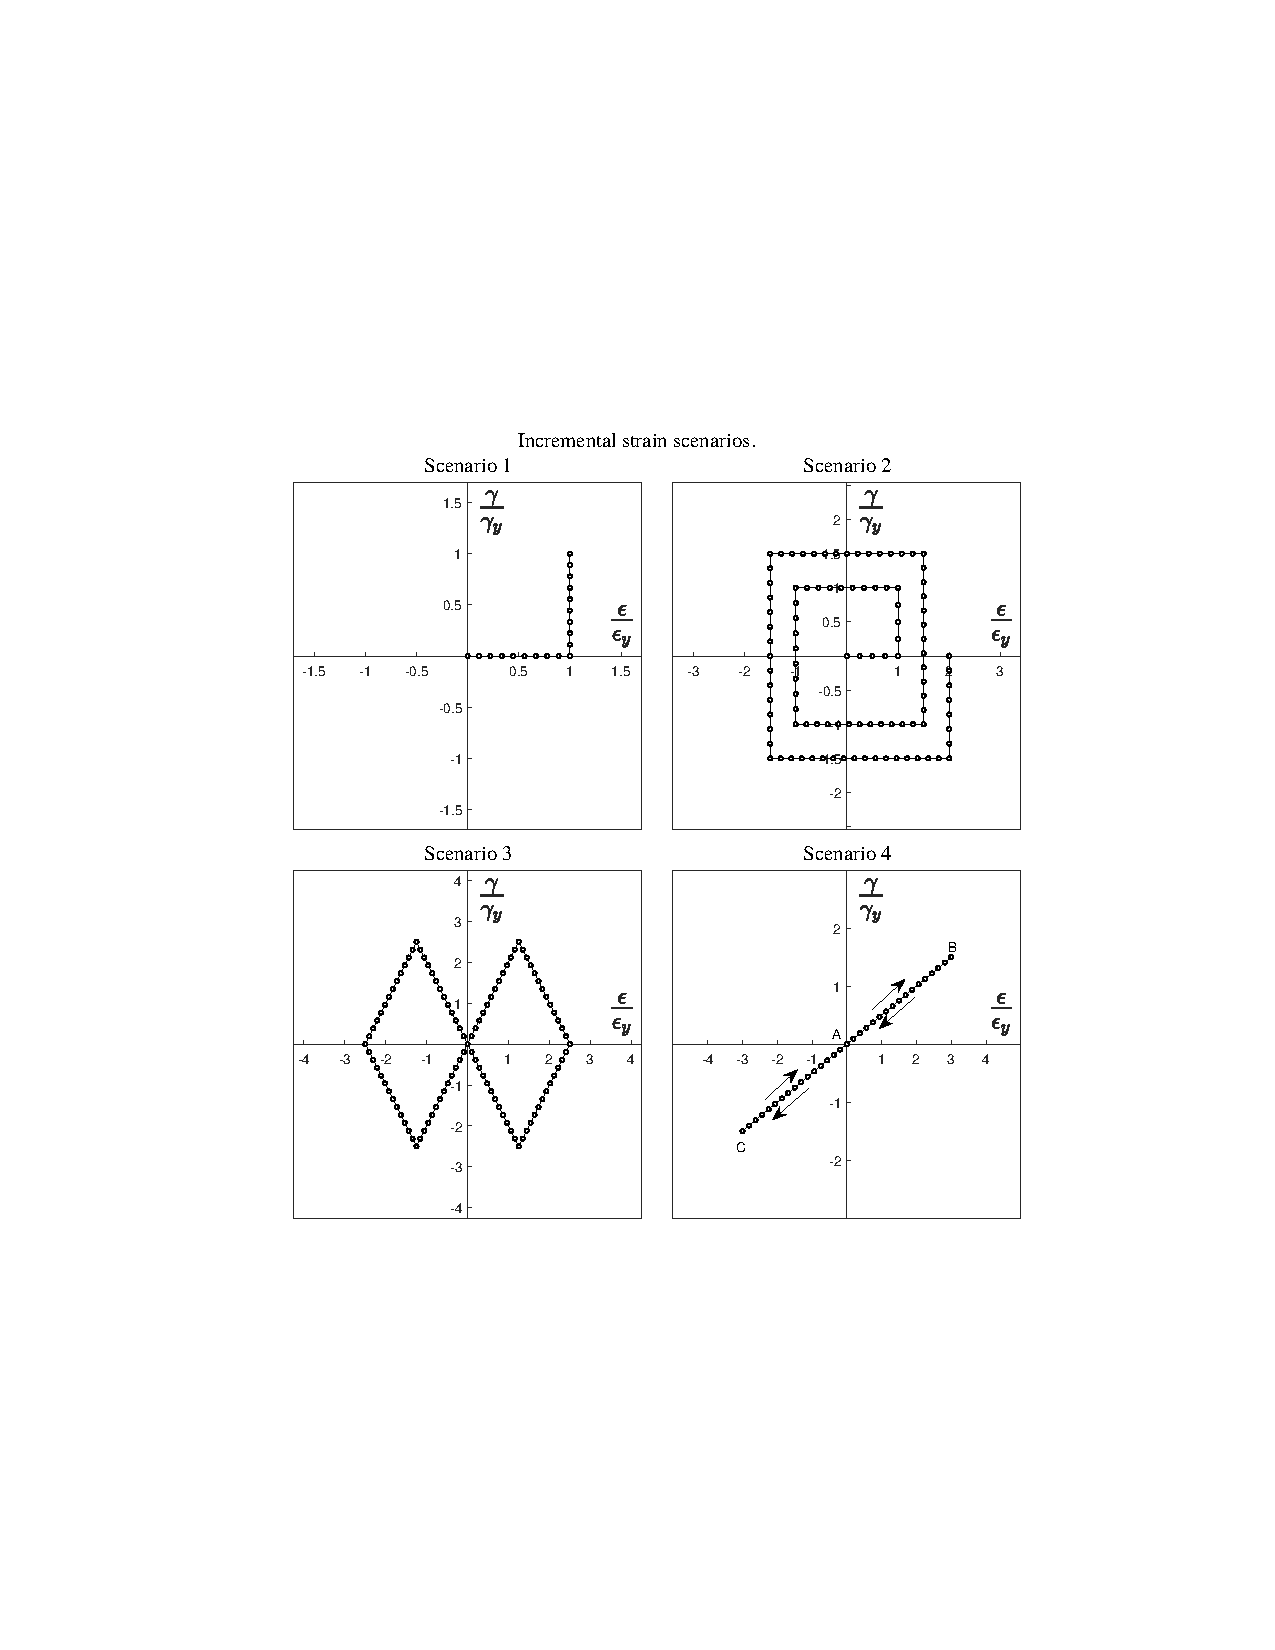
\includegraphics[scale=0.7]{FIG20_STRAIN_HISTORIES}
	\caption{The four different strain histories imposed, with the unstresses 
		configuration as initial point.}
	\label{fig:FIG20_STRAIN_HISTORIES}
\end{figure}

As can be seen from the Tables \ref{table:TABLE_1}-\ref{table:TABLE_4}, the 
proposed scheme offers significant speed-up compared to the other two methods. 
It should be highlighted that the 3D algorithm outperforms the one proposed by 
Simo because a perfectly plastic $J_2$ was used. In 
general, it too would require internal iterations to determine $\lambda$, in 
addition to the outer level Newton procedure to enforce the stress constraints. 
For Scenario 4, shown in Table \ref{table:TABLE_4}, both the 3D and plane 
stress algorithms did $[440,\ 188,\ 84,\ 62]$ elastic iterations corresponding 
to values of parameter $\alpha$: $[0.10,\ 0.25,\ 0.40,\ 0.50]$.




\begin{table}   % TABLE 1 - EXAMPLE 2
	\setlength{\tabcolsep}{9pt}
	\caption{Results for Scenario 1, perfect plasticity.}
	%	\noindent\makebox[\textwidth]{
		\begin{tabular}{@ {}lccccccccc@ {}}\toprule\toprule[0.4pt]
			Algorithm & Exact & \multicolumn{2}{c}{$\alpha=0.10$} & 
			\multicolumn{2}{c}{$\alpha=0.25$} &
			\multicolumn{2}{c}{$\alpha=0.40$}  &
			\multicolumn{2}{c}{$\alpha=0.50$}\\
			\cmidrule(r{0.60cm}l{0.40cm}){3-4} 
			\cmidrule(r{0.43cm}l{0.42cm}){5-6}
			\cmidrule(r{0.43cm}l{0.42cm}){7-8} 
			\cmidrule(r{0.10cm}l{0.45cm}){9-10}
			& $(\sigma_{11},\sigma_{12})$ & $t$\textsuperscript{a} & $N_i$ & 
			$t$ & $N_i$ & 
			$t$ & $N_i$ & $t$ & $N_i$\\
			\midrule[0.5pt]
			Proposed & {\small (1.617,1.023)} & 0.57 & 29 & 0.44 & 13 & 0.40 & 
			8 & 0.38 &  5 \\
			3D & & 1.40 & 46(20) & 0.83 & 20(8) & 0.65 & 11(4) & 0.56 
			& 6(2) \\
			Simo     &  & 1.64 & 165(19) & 1.13 & 88(7) & 0.96 & 64(3) & 0.83 & 
			55(1) \\
			\cmidrule{3-10}
			Error(\%)\textsuperscript{b}     &  & \multicolumn{2}{c}{$1.32$} & 
			\multicolumn{2}{c}{$3.00$} & \multicolumn{2}{c}{$5.16$} & 
			\multicolumn{2}{c}{$8.05$}\\
			\bottomrule\bottomrule[0.5pt]\addlinespace[3pt]
			\multicolumn{8}{l}{\textsuperscript{a} Measured in $\times 10^{-3}$ 
				sec.}\\
			\multicolumn{8}{l}{\textsuperscript{b} Relative error in converged 
				stress per increment scenario.}
		\end{tabular}
		\label{table:TABLE_1}
		%	}
\end{table}

\begin{table}   % TABLE 2 - EXAMPLE 2
	\setlength{\tabcolsep}{6.5pt}
	\caption{Results for Scenario 2, perfect plasticity.}
	%	\noindent\makebox[\textwidth]{
		\begin{tabular}{@ {}lccccccccc@ {}}\toprule[0.5pt]\toprule
			Algorithm & Exact & \multicolumn{2}{c}{$\alpha=0.10$} & 
			\multicolumn{2}{c}{$\alpha=0.25$} &
			\multicolumn{2}{c}{$\alpha=0.40$}  &
			\multicolumn{2}{c}{$\alpha=0.50$}\\
			\cmidrule(r{0.63cm}l{0.35cm}){3-4} 
			\cmidrule(r{0.63cm}l{0.40cm}){5-6}
			\cmidrule(r{0.52cm}l{0.40cm}){7-8} 
			\cmidrule(r{0.30cm}l{0.33cm}){9-10}
			& $(\sigma_{11},\sigma_{12})$ & $t$\textsuperscript{a} & $N_i$ & 
			$t$ & $N_i$ & 
			$t$ & $N_i$ & $t$ & $N_i$\\
			\midrule[0.5pt]
			Proposed & {\small (1.173,1.208)} & 0.33 & 524 & 0.16 & 234 & 0.10 
			& 144 & 0.08 & 108 \\
			3D    &                 & 1.24 & 849(97) & 0.61 & 394(40) & 0.31 
			& 196(17) & 0.23 & 143(11) \\
			Simo     &  & 2.09 & 2791(96) & 1.17 & 1363(39) & 0.57 
			& 790(15) & 0.42& 596(10) \\
			\cmidrule{3-10}
			Error(\%)     &  & \multicolumn{2}{c}{$2.32$} & 
			\multicolumn{2}{c}{$5.00$} & \multicolumn{2}{c}{$10.10$} & 
			\multicolumn{2}{c}{$13.35$}\\
			\bottomrule[0.5pt]\bottomrule[0.5pt]\addlinespace[3pt]
			\multicolumn{8}{l}{\textsuperscript{a} Numbers in executiont time 
				columns are measured in $\times 10^{-2}$ s.}\\
		\end{tabular}
		\label{table:TABLE_2}
		%	}
\end{table}

\begin{table}    % TABLE 3 - EXAMPLE 2
	\caption{Results for Scenario 3, perfect plasticity.}
	%\noindent\makebox[\textwidth]{
		\begin{tabular}{@ {}lccccccccc@ {}}\toprule\toprule
			Algorithm & Exact & \multicolumn{2}{c}{$\alpha=0.10$} & 
			\multicolumn{2}{c}{$\alpha=0.25$} &
			\multicolumn{2}{c}{$\alpha=0.40$}  &
			\multicolumn{2}{c}{$\alpha=0.50$}\\
			\cmidrule(r{0.65cm}l{0.30cm}){3-4} 
			\cmidrule(r{0.60cm}l{0.30cm}){5-6}
			\cmidrule(r{0.52cm}l{0.37cm}){7-8} 
			\cmidrule(r{0.33cm}l{0.30cm}){9-10}
			& $(\sigma_{11},\sigma_{12})$ & $t$\textsuperscript{a} & $N_i$ & 
			$t$ & $N_i$ & $t$ & $N_i$ & $t$ & $N_i$\\
			\midrule[0.8pt]
			Proposed & {\small (1.628,1.018)} & 0.35 & 546 & 0.16 & 237 & 0.11 
			& 147 & 0.09 &  126 \\
			3D &  & 1.15 & 920(115) & 0.61 & 405(50) & 0.31 & 194(22) & 0.29 & 
			167(16) \\
			Simo     &  & 2.20 & 2711(114) & 1.42 & 1307(50) & 0.55 & 789(20) & 
			0.48 & 685(14) \\
			\cmidrule{3-10}
			Error(\%)     &  & \multicolumn{2}{c}{$1.15$} & 
			\multicolumn{2}{c}{$2.51$} & \multicolumn{2}{c}{$5.40$} & 
			\multicolumn{2}{c}{$5.80$}\\
			\bottomrule\bottomrule[0.5pt]\addlinespace[3pt]
			\multicolumn{8}{l}{\textsuperscript{a} Numbers in execution time 
				columns are measured in $\times 10^{-2}$ s.}
		\end{tabular}
		\label{table:TABLE_3}
		%	}
\end{table}

\begin{table}
	\setlength{\tabcolsep}{9.7pt}
	\caption{Results for Scenario 4, five cycles, perfect plasticity. One 
		cycle: A-B-C-A.}
	%\noindent\makebox[\textwidth]{
		\begin{tabular}{@ {}lccccccccc@ {}}\toprule\toprule[0.5pt]
			Algorithm & Exact &
			\multicolumn{2}{c}{$\alpha=0.10$} &
			\multicolumn{2}{c}{$\alpha=0.25$} &
			\multicolumn{2}{c}{$\alpha=0.40$} &
			\multicolumn{2}{c}{$\alpha=0.50$}\\
			\cmidrule(r{0.38cm}l{0.40cm}){3-4} 
			\cmidrule(r{0.43cm}l{0.45cm}){5-6}
			\cmidrule(r{0.43cm}l{0.45cm}){7-8} 
			\cmidrule(r{0.09cm}l{0.43cm}){9-10}
			& $(\sigma_{11},\sigma_{12})$ & $t$\textsuperscript{a} & $N_i$ & 
			$t$ & $N_i$ & $t$ & $N_i$ & $t$ & $N_i$\\
			\midrule[0.5pt]
			Proposed & {\small (2.196,0.559)} & 0.92 & 1500 & 0.44 & 678 & 0.22 
			& 392 & 0.19  & 345 \\
			3D &                    & 3.50 & 2500 & 1.61 & 1130 & 0.77 & 490 & 
			0.69 & 445 \\
			Simo     &                        & 5.20 & 7497 & 2.93 & 4519 & 
			1.60 & 2352 & 1.38& 2122 \\
			\cmidrule{3-10}
			Error(\%)     &  & \multicolumn{2}{c}{$0.19$} & 
			\multicolumn{2}{c}{$0.40$} & \multicolumn{2}{c}{$0.84$} & 
			\multicolumn{2}{c}{$0.91$}\\
			\bottomrule\bottomrule[0.5pt]\addlinespace[3pt]
			\multicolumn{8}{l}{\textsuperscript{a} Numbers in execution time 
				columns are measured in $\times 10^{-2}$ s.}
		\end{tabular}
		\label{table:TABLE_4}
		
		%	}
\end{table}


%%%%%%%%%%%%%%%%%%%%  EXAMPLE 3 %%%%%%%%%%%%%%%%%%%%%%%%%%%%%%%%
\subsection{Plastic Collapse of a Doubly Clamped Beam}

In this example we investigate the collapse load of a doubly clamped beam, 
shown in Fig. \ref{fig:FIG21_CLAMPED_BEAM}, for two slenderness rations, 
$L^{}/h$: $20$ and $4$, where $h$ is 
the cross-section height. We conduct 
analysis using both uncoupled and coupled, multiaxial, constitutive models at 
the fiber level and compare result, for each case, with the lower bound 
collapse load as predicted by limit analysis.

 In addition, we showcase the 
influence of numerical quadrature in predicting the analytical solution in the 
slender case. More specifically, we compare Gauss-Legendre and Gauss-Lobatto 
quadratures. The quadrature rule used is crucial for both flexibility-based 
beam elements and the hybrid one presented and used herein, since, in both 
formulations, accuracy relies more on the precision of integration rather than 
mesh density. Lastly, each cross-section is discretized into 15 layers.

The shear strain distribution function, $k_q\varphi(X_2)$, is assumed to be 
parabolic and defined as follows:
\begin{equation}
	\varphi(X_2) = (1-4\frac{X_2^2}{h^2})
	\label{eq:SHEAR_DISTR_FUN}
\end{equation}
\noindent where $k_q$ is a parameter introduced in order to establish shear 
strain energy equivalnce between assumed and exact distributions. For that 
matter, it is convenient to consider the uniform shear strain-average force 
hypothesis coupled with the corresponding shear coefficient as a representation 
of the exact one, assuming elastic behavior:
\begin{equation}
	\mathcal{U}_{shear}^{exact}=k_s\mathcal{U}_{shear}^{unif} = 
	\mathcal{U}_{shear}^{quad}\Longleftrightarrow 
	\frac{1}{2}k_sGA\gamma ^2=\frac{1}{2}G k_q^2\bigg(\int_A \varphi(X_2)^2 dA 
	\bigg) \gamma ^2
	\label{eq:SHEAR_COEFF}
\end{equation}
\noindent where $k_s$ is the shear coefficient for uniform shear strain 
assumption. For rectangular sections with $\nu=0.3$, 
$k_s=0.886$ and solving eq. \ref{eq:SHEAR_COEFF} for $k_q$ we 
get:
\begin{equation}
	k_q = \sqrt{\frac{k_s A}{\int_A \varphi(X_2)^2 dA}}
	\label{eq:QUAD_COEFF}
\end{equation}

A first observation from fig \ref{fig:FIG22_EQUILIBRIUM_PATHS} is that 
Gauss-Legendre quadrature tends to overestimate the capacity load in both edges 
of the slenderness spectrum and . Gauss-Lobatto quadrature, in contrast, is 
more accurate and converges to the ``exact'' capacity from ``below''. In 
addition, it provides accuracy with juts 5 quadrature points whereas even with 
9 points, Gauss-Legendre still is not as accurate and converges from ``above''. 
The results are in agreement with the ones reported by Papachristidis et 
al.\cite{Papachristidis2010} in a similar investigation but using a flexibility 
element.

When it comes to the influence of slenderness in the plastic capacity, the 
collapse 
load for the $L^{}/h$ case predicted by the multiaxial constitutive law is 
lower than the one based on limit analysis. Interestingly, the uncoupled 
constitutive law results in a purely flexural collapse mode, thus yielding a 
ultimate load coinciding with the theoretical from limit analysis. When the 
beam is slender, both coupled and uncoupled constitutive laws result, 
expectably, in a flexure-dominant mode. The results are summarized in Table 
\ref{table:TABLE_5} and Fig. \ref{fig:FIG22_EQUILIBRIUM_PATHS}. In Fig. 
\ref{fig:FIG23} the stress distributions for $\sigma_{11}$, $\sigma_{12}$ and 
the von Mises stress, $\sigma_{VM}=\sqrt{3J_2}$ are presented at three 
different load levels indicate dy point A, B and C (see Fig. 
\ref{fig:FIG22_B}). 
The plastic zone propagation is also shown. We observe that the lower 
capacity as captured by the multiaxial model in the $L^{}/h=4$ case, which Fig. 
\ref{fig:FIG23} pertains to, is due to shear plastification of the -shrinking- 
elastic core.

\begin{figure}
	\centering
	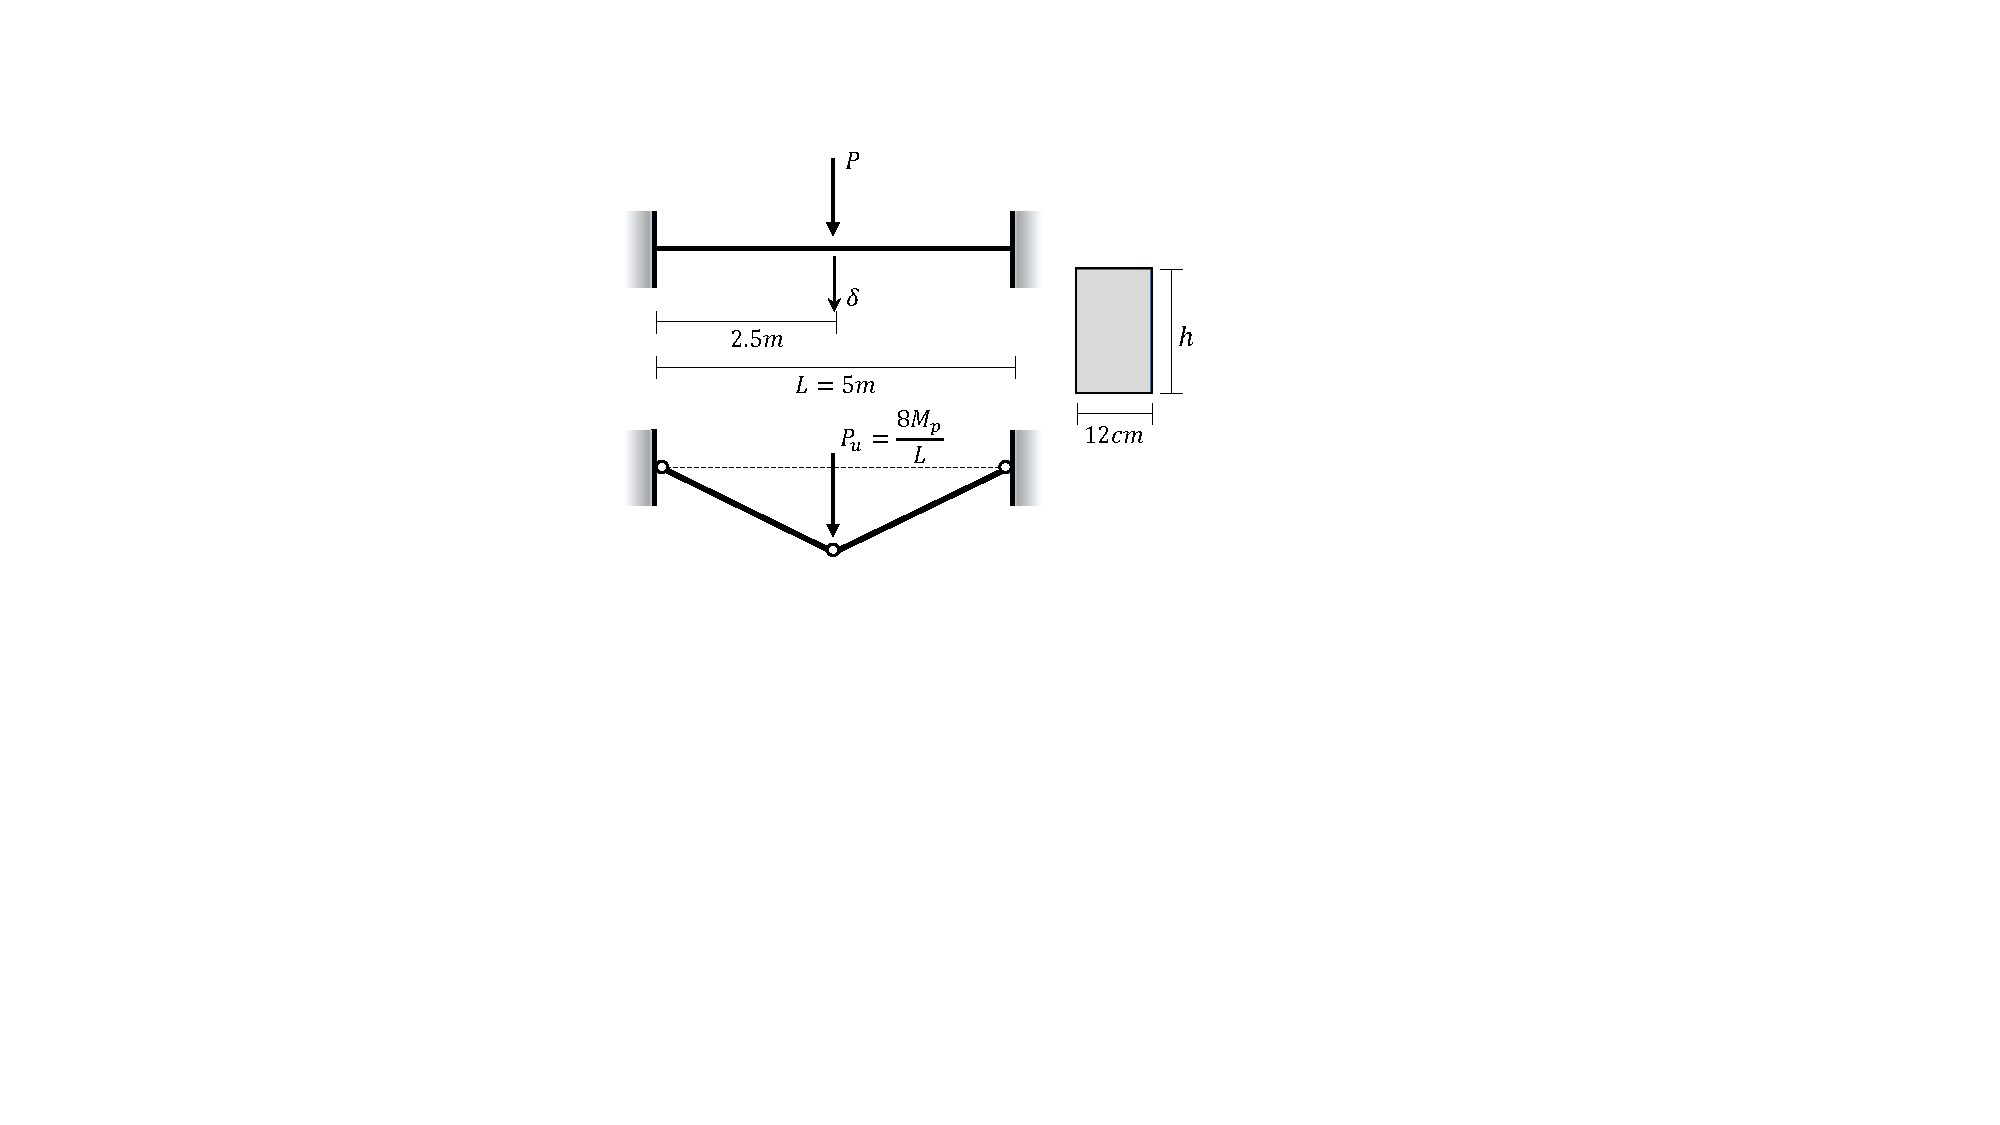
\includegraphics[scale=0.9]{FIG21_CLAMPED_BEAM}
	\caption{Geometry, initial and final configuration of clamped beam, along 
		with cross-section dimensions.}
	\label{fig:FIG21_CLAMPED_BEAM}
\end{figure}

\noindent\makebox[\textwidth][c]{
	\begin{minipage}{0.7\textwidth}
		\vskip15pt
		\captionof{table}{Collapse moments and loads for clamped beam.}
		\begin{tabular}{@ {}ccccc@ 
				{}}\toprule[0.4pt]\toprule[0.4pt]\addlinespace[-2pt]
			&  & \multicolumn{3}{c}{Collapse load, 
				$P_u(kN)$\textsuperscript{a}}\\ 
			\cmidrule{3-5}
			$L^{}/h$ & $M_p(kN\cdot m)$ & Limit Analysis & Uncoupled & Coupled\\
			\midrule[0.5pt]\addlinespace[-2pt]
			$20$ & $3.75\cdot 10^2$ & $6.00\cdot 10^2$ & $\approx 6.00\cdot 
			10^2$ & $\approx 6.00\cdot 10^2$\\ \addlinespace[-2pt]
			$4$  & $9.37\cdot 10^3$ & $1.50\cdot 10^4$ & $\approx 1.50\cdot 
			10^4$ & $\approx 1.43\cdot 10^4$\\ \addlinespace[-2pt]
			\bottomrule[0.4pt]\bottomrule[0.4pt]\addlinespace[-3pt]
			\multicolumn{5}{l}{\small Material data: $E=200\ GPa$, 
				$\sigma_y=200\ 
				MPa$.}\\ \addlinespace[-9pt]
			\multicolumn{5}{l}{\textsuperscript{a} \small For coupled and 
				uncoupled loads, 5 Gauss-Lobatto points are assumed.}
		\end{tabular}
		
		\label{table:TABLE_5}
	\end{minipage}
}

\begin{figure}[t]
	\centering
	\subfloat[$L^{}/h=20$]{%
		\hspace{-0.2cm}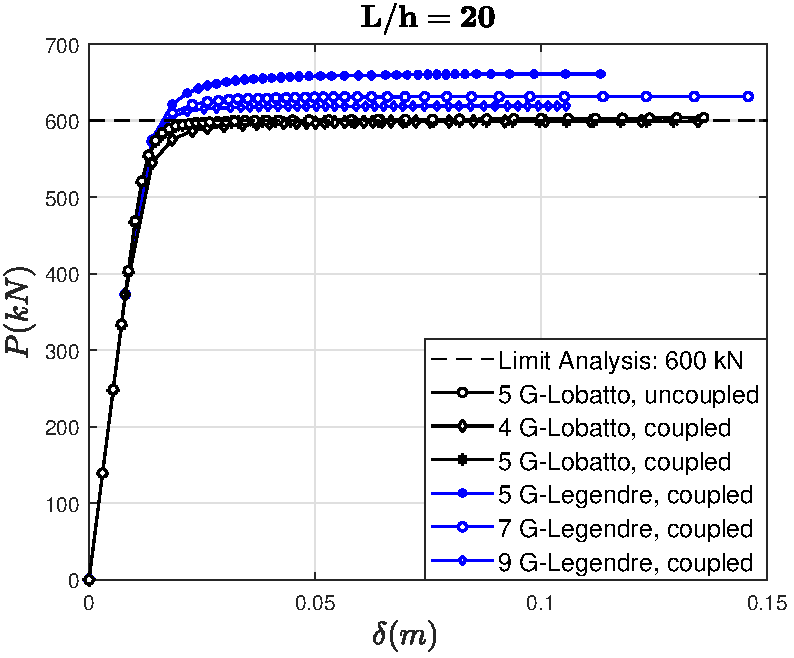
\includegraphics[width=0.45\textwidth]{FIG22_A_CLAMPED_LH20}%
		\label{fig:FIG22_A}%
	}
	\subfloat[$L^{}/h=4$]{%
		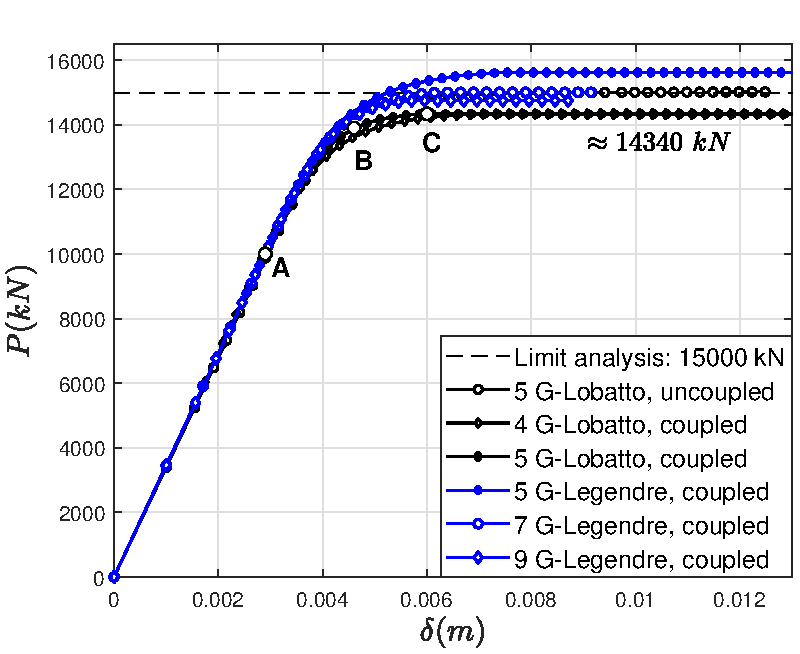
\includegraphics[width=0.45\textwidth]{FIG22_B_CLAMPED_LH4}%
		\label{fig:FIG22_B}%
	}
	\caption{Load-deflection plots for different slenderness ratios. Influence 
		of quadrature type and number of points.}
	\label{fig:FIG22_EQUILIBRIUM_PATHS}
\end{figure} 

\begin{figure}
	\centering
	\setlength\tabcolsep{1pt}
	%\settowidth\rotheadsize{Plastification}
	\begin{tabular}{c|ccc}
		& \textbf{A} : $P=10000\ kN$  & \textbf{B} : $P=13900\ 
		kN$              
		& \textbf{C} : $P = 14340\ kN$\\
		\midrule
		P.Z.         & \sprofs{FIG23_PlastP10000.pdf}     & 
		\sprofs{FIG23_PlastP13900.pdf}     & \sprofs{FIG23_PlastP14340.pdf}\\
		$\sigma_{VM}$& \sprofs{FIG23_PlastP10000_VM.pdf}  & 
		\sprofs{FIG23_PlastP13900_VM.pdf}  & \sprofs{FIG23_PlastP14340_VM.pdf}\\
		$\sigma_{11}$     & \sprofs{FIG23_PlastP10000_SXX.pdf} & 
		\sprofs{FIG23_PlastP13900_SXX.pdf} & 
		\sprofs{FIG23_PlastP14340_SXX.pdf}\\
		$\sigma_{12}$       & \sprofs{FIG23_PlastP10000_SXY.pdf} & 
		\sprofs{FIG23_PlastP13900_SXY.pdf} & \sprofs{FIG23_PlastP14340_SXY.pdf}
	\end{tabular}
	\caption{Case $L^{}/h=4$. Spread of Plastic Zone (P.Z.) and stress 
		distribution for von 
		Mises, axial and shear stress at three different load levels.}
	\label{fig:FIG23}
\end{figure}

\clearpage
%%%%%%%%%%%%%%%%%%%%  EXAMPLE 4 %%%%%%%%%%%%%%%%%%%%%%%%%%%%%%%%
\subsection{Cyclic Loading of Shear Link}\label{CH3EX4}

In this example we are examining the response of a metallic shear link 
(Fig.\ref{fig:FIG24A}) 
with a symmetric wide flange cross-section under displacement-controlled cyclic 
loading. The specimen we are concerned with was part of an experimental 
investigation by Hjelmstad \& Popov\cite{Hjelmstad1983} and later was 
numerically analyzed by Saritas \& Filippou\cite{Saritas2009} using a mixed 
beam element formulation with shear-flexure interaction at the fiber level. In 
our analsys the specimen was modelled using one hybrid element with 5 
Gauss-Lobatto points and 31 layers at each section with five layers on each 
flange. 

The specimen length is $L=28$ in. and the cross-section type is W $18\ \times\ 
40$ with basic dimensions 
specified as follows: total height $h=17.88$ in., flange width $b=5.985$ in., 
web and flange thickness, $t_w=0.314$ in. and $t_F=0.521$ in. respectively. The 
material properties are summarized in Table \ref{table:TABLE6}, while the 
displacement history, in 
accordance with Hjelmstad \& Popov's experiment, is shown in 
Fig.\ref{fig:FIG24B} The plastic 
modulus corresponding to linear kinematic hardening was determined from  
uniaxial data to be $H_{kin}=102$ kips/in${}^2$. A nonlinear hardening law was 
specified for the isotropic part, which is given as follows:
\begin{equation}
	q(e^{pl}) = \sigma_y + C(1-\text{exp}(-\rho e^{pl}))
	\label{eq:NONLIN_ISOTROPIC_HARD}
\end{equation}
\noindent where $C=\sigma_u-\sigma_y$, $\sigma_u$, $\sigma_y$ the ultimate and 
yield stresses respectively and $\epsilon_u$, $\epsilon_y$ the corresponding 
strains. Parameter $\rho$ is specified as 
$\rho=20$ in this analysis. The shear strain distribution is again assumed to 
be quadratic, where $k_s=0.466$ and, using eq. (\ref{eq:QUAD_COEFF}),  
$k_q=1.33$.

\begin{figure}[t]
	\centering
	\subfloat[Structure.]{
		\begin{minipage}[c]{0.4\linewidth}
			%\captionsetup{type=figure}
			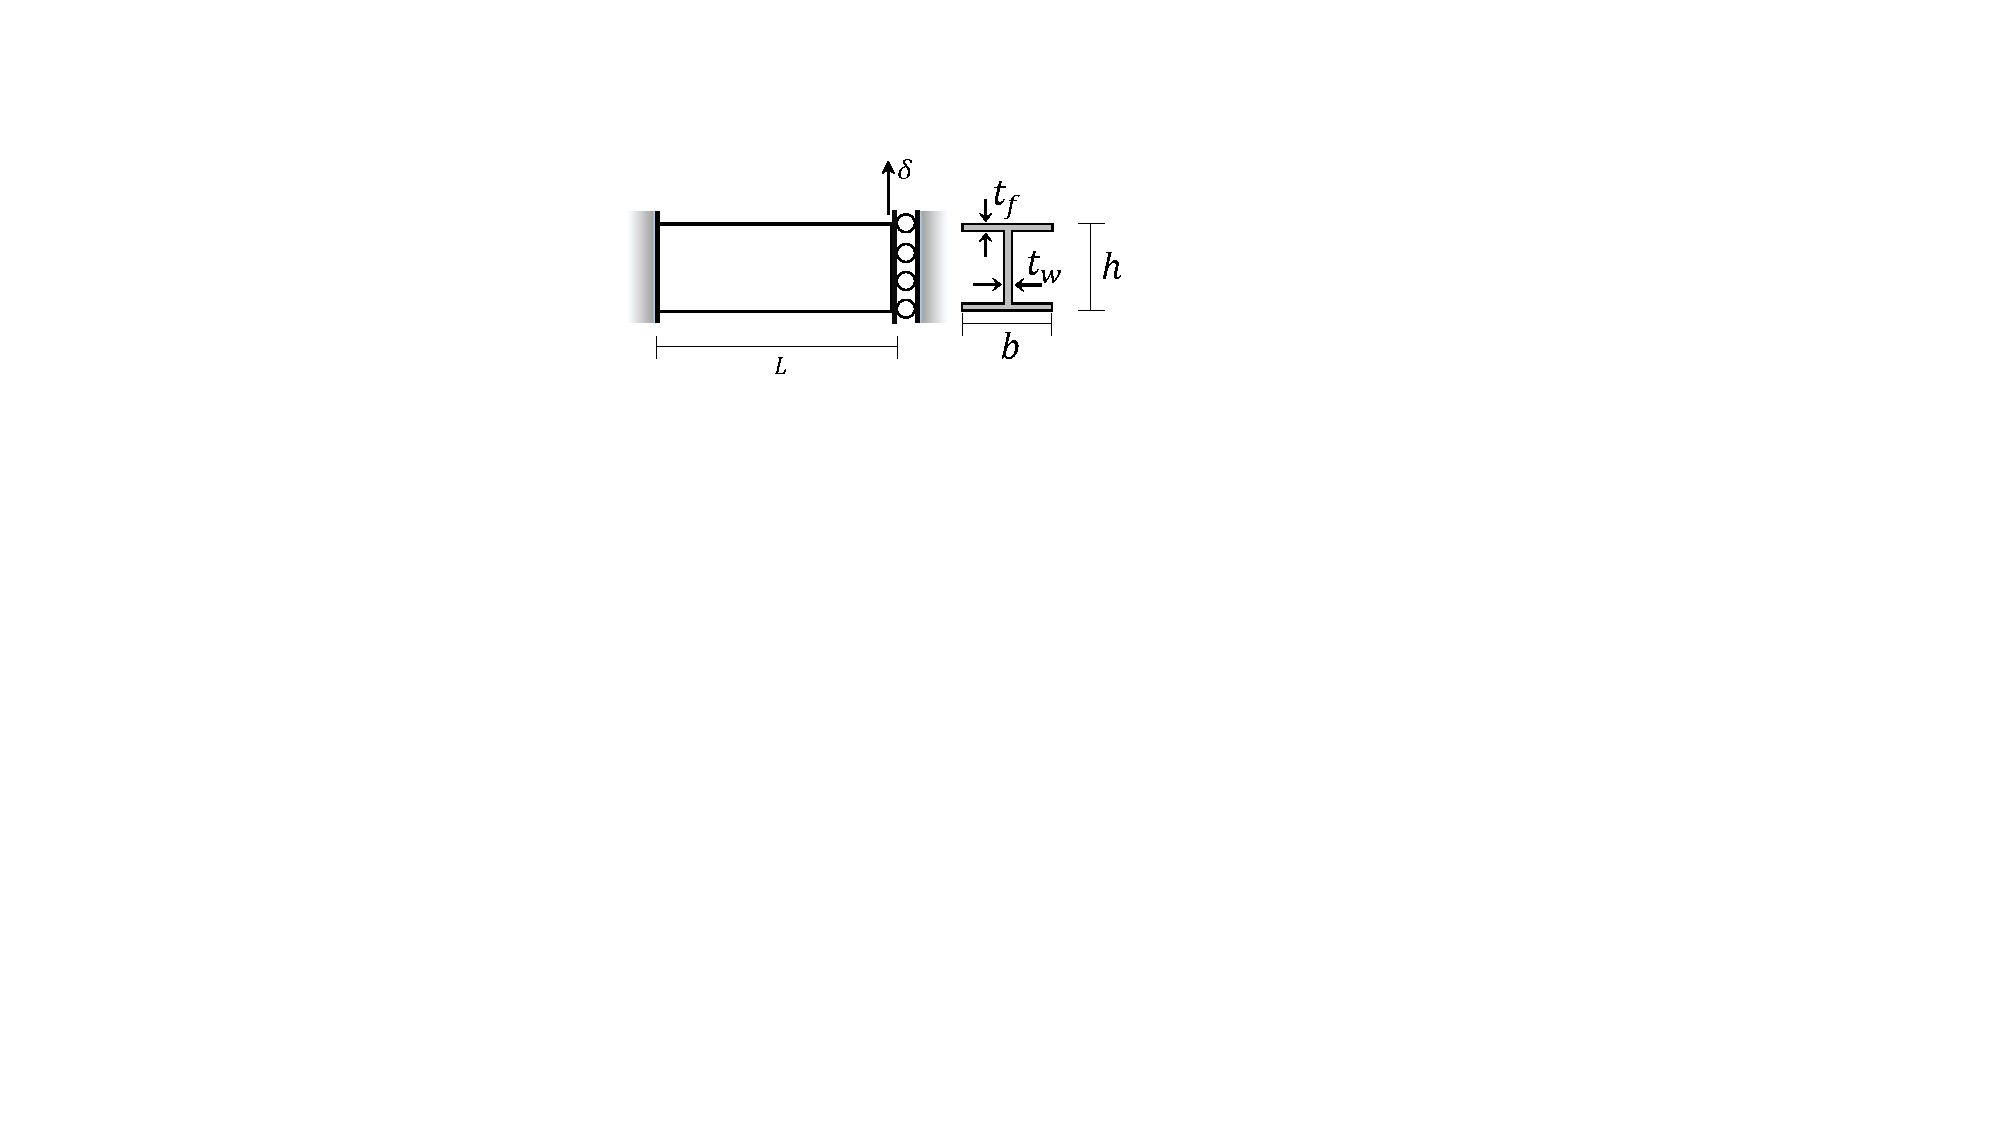
\includegraphics[scale=0.8]{FIG24_Structure}%
			%\caption{Structure.}
			\label{fig:FIG24A}%
		\end{minipage}
	}
	%\subfloat[Structure.]{%
		%	
		%\hspace{-0.2cm}\includegraphics[width=0.45\textwidth]{FIG11_Structure}%
		%	\label{fig:FIG11A}%
		%	}
	\subfloat[Displacement-controlled loading history.]{%
		\hspace{0.3cm}\begin{minipage}{0.55\linewidth}
			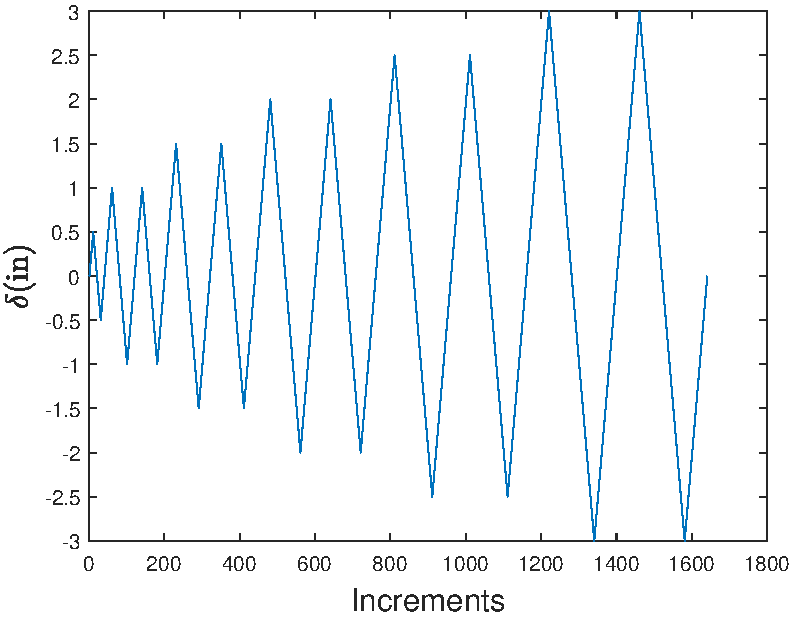
\includegraphics[scale=0.6]{FIG24_DISPHIST}%
			\label{fig:FIG24B}%
		\end{minipage}
		%\includegraphics[width=0.45\textwidth]{FIG11_DISPHIST}%
		%\label{fig:FIG11B}%
	}
	\caption{Geometry of the specimen and displacement-controlled loading 
		history.}
	\label{fig:FIG24}
\end{figure} 

\begin{table}[b]
	\centering
	\begin{minipage}{0.8\linewidth}
		\caption{Material properties for Example \ref{CH3EX4}.}
		\begin{tabular}{ccccccc}
			\toprule\toprule
			\vtop{\hbox{\strut \hspace{.25cm}Section}\hbox{\strut W 
			$18\times40$}} 
			& \vtop{\hbox{\strut \hspace{0.5cm}$\sigma_y$}\hbox{\strut 
					($\text{kips}^{}/\text{in}^2$)}}  &         
					\vtop{\hbox{\strut 
					\hspace{0.5cm}$\sigma_u$}\hbox{\strut 
					($\text{kips}^{}/\text{in}^2$)}} &
			\vtop{\hbox{\strut \hspace{2.5pt}$\epsilon_y$}\hbox{\strut (\%)}} & 
			\vtop{\hbox{\strut \hspace{2.5pt}$\epsilon_u$}\hbox{\strut (\%)}} 
			&\vtop{\hbox{\strut \hspace{0.5cm}$E$}\hbox{\strut 
					($\text{kips}^{}/\text{in}^2$)}} & \vtop{\hbox{\strut 
					\hspace{0.4cm}$H_{kin}$}\hbox{\strut 
					($\text{kips}^{}/\text{in}^2$)}} \\
			\midrule
			Web & 39.5 & 60.1 & 1.8 & 22 & 28,300 & 102 \\
			Flange & 35.0 & 58.5 & 1.4 & 24 & 28,000 & 102\\
			\bottomrule\bottomrule
		\end{tabular}
		\label{table:TABLE6}
	\end{minipage}
\end{table}

\begin{figure}[t]
	\centering
	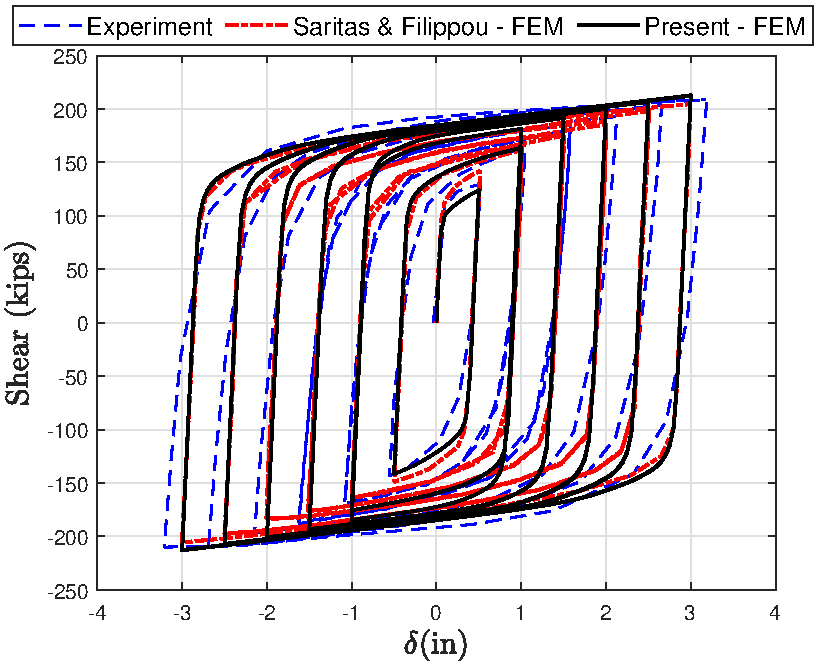
\includegraphics[scale=0.9]{FIG25_HISTORIES}
	\caption{Experimental and numerical results for the specimen.}
	\label{fig:FIG25}
\end{figure}

As can be seen from Fig.\ref{fig:FIG25}, during the first cycle we have 
satisfactory agreement between the present analysis and the experimental 
result, while for all cycles after the third, we have almost excellent match 
between all cyclic histories shown. For the second and third cycles, with peak 
displacement at $1$ inch, the present analysis exhibits a more abrupt yielding. 
This happens because most of the core becomes plastified within a smaller range 
of increments. While the hardening rules adopted might affect this behavior, it 
is the assumed shear strain distribution that playes a central role in 
transitioning from the elastic to plastic regime. Formulations that also 
consider shear stress distribution functions along the cross-section, section 
warping or even more accurate shear strain distribution models can definitely 
improve the approximation. We can also observe that both numerical models show 
identical accuracy during the unloading steps and a noticable discrepancy with 
the experimental analysis. As explained in \cite{Saritas2009}, this is due to 
improper restraint of the specimen during the experiment.

Performance analysis of the three different return-mapping schemes is also 
conducted for this example, where now we will examine the total number of 
constitutive iterations during the whole history of the imposed displacement. 
This helps highlight the significant acceleration the proposed algorithm offers 
when a complex analysis that involves nonlinear response of an element 
comprised of different sections, each of which is discretized in several 
layers. The results when we use the three-dimensional/axisymmetric, Simo's 
plane stress and the proposed algorithm are shown in Fig. \ref{fig:FIG_BARS}. 
As mentioned earlier, the constitutive model even tends to favor the 
three-dimensional algorithm since the plastic correction reduces to the 
so-called radial return for this particular constitutive model. However, in a 
more general setting where nonlinear hardening or a different material model is 
used, the perfromance differentials between the proposed scheme and the its 
three-dimensional counterpart would be even more pronounced.

 \begin{figure}[t]
 	\centering
 	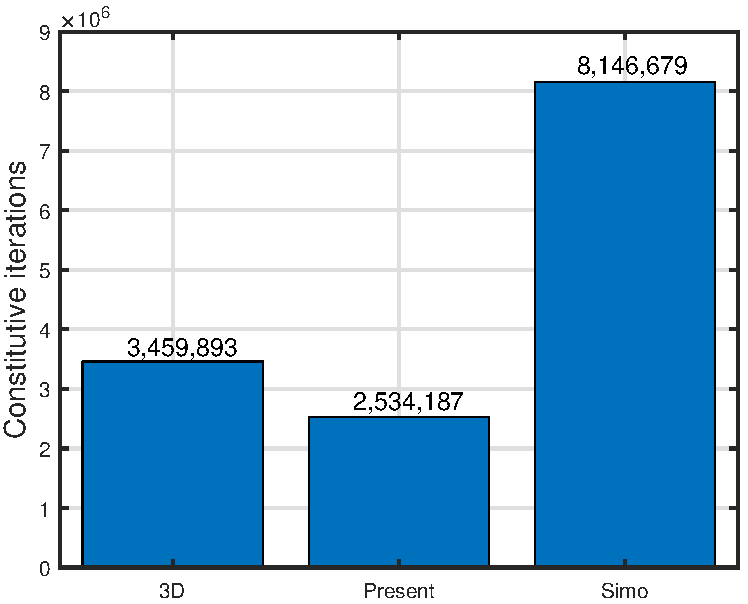
\includegraphics[scale=0.9]{FIG_BARS}
 	\caption{Performance of the three different return-mapping algorithms 
 	applied for the section state determination of the shear link under the 
 	imposed displacement history.}
 	\label{fig:FIG_BARS}
 \end{figure}
%%%%%%%%%%%%%%%%%%%%  EXAMPLE 5 %%%%%%%%%%%%%%%%%%%%%%%%%%%%%%%%
\subsection{Elastoplastic Post-Buckling Behavior of Two-Beam Structure}

This problem has been previously analyzed in \cite{Argyris1982,Ridha1971}. The 
structure, shown in Fig. \ref{fig:FIG26_STRUCTURE}, enters its inelastic regime 
imediatelly after the buckling 
load is reached, whereby point B starts moving inwards. In 
Fig. \ref{fig:FIG26_COMPARISON} we compare the 
results we get using just 3 hybrid elements and 5 Gauss-Lobatto points in each 
element with Argyris et al.\cite{Argyris1982}. In addition, we include the 
inelastic analysis, which demonstrates that plastification starts immediately 
after then instability. The material and geometric data are shown in 
Table \ref{table:TABLE7}. Again, we highlight the impact of a coupled 
multiaxial law by 
investigating a variation of this problem. For all cases, inelastic response 
with kinematic hardening is assumed. The convergence rates in residual norm and 
energy norms for the case of thick members is also shown in Tables 
\ref{table:TABLE8}, \ref{table:TABLE9}. In Fig. \ref{fig:RATES} we also show 
plots of convergence rates for the global Newton method when using the 
consistent and continuous tangent respectively for two representative steps. It 
is evident that use of the continuous tangent modulus slows down convergence 
significantly.

As can be seen from 
Fig. \ref{fig:FIG27_PLASTIC} for the inelastc analysis of 
the thick member variation, the equilibrium paths corresponding to a coupled 
and uncoupled constitutive law tend to diverge shortly after the start of 
plastic deformation.

\begin{table}
	\centering
 	\begin{minipage}{0.7\textwidth}
 		%\vskip-10pt
 		\caption{Member geometric and material data.}
 		\label{table:TABLE7}
 		\begin{tabular}{@ {}ccccccc@ {}}\toprule\toprule
 			Member & $E (\frac{\text{kN}}{\text{cm}^2})$ & 
 			$H_{kin}(\frac{\text{kN}}{\text{cm}^2})$ & 
 			$\sigma_y(\frac{\text{kN}}{\text{cm}^2})$ & $h_s(\text{cm})$ & 
 			$h_t(\text{cm})$ & $b(\text{cm})$\\
 			\midrule[0.5pt]
 			\circled{1} & $6.86\times 10^3$ & $2.84\times 10^2$ & $26.20$ & 
 			$1.91$ & $8.00$ & $2.54$ \\ \addlinespace[3pt]
 			\circled{2} & $6.86\times 10^3$ & $2.84\times 10^2$ & $33.10$ & 
 			$1.91$ & $8.00$ & $2.54$ \\
 			\bottomrule\bottomrule[0.5pt]\addlinespace[3pt]
 		\end{tabular}
 	\end{minipage}
\end{table}

\clearpage
\begin{figure}[t]
	\centering
	\subfloat[Structure.]{%
		\hspace{-0.2cm}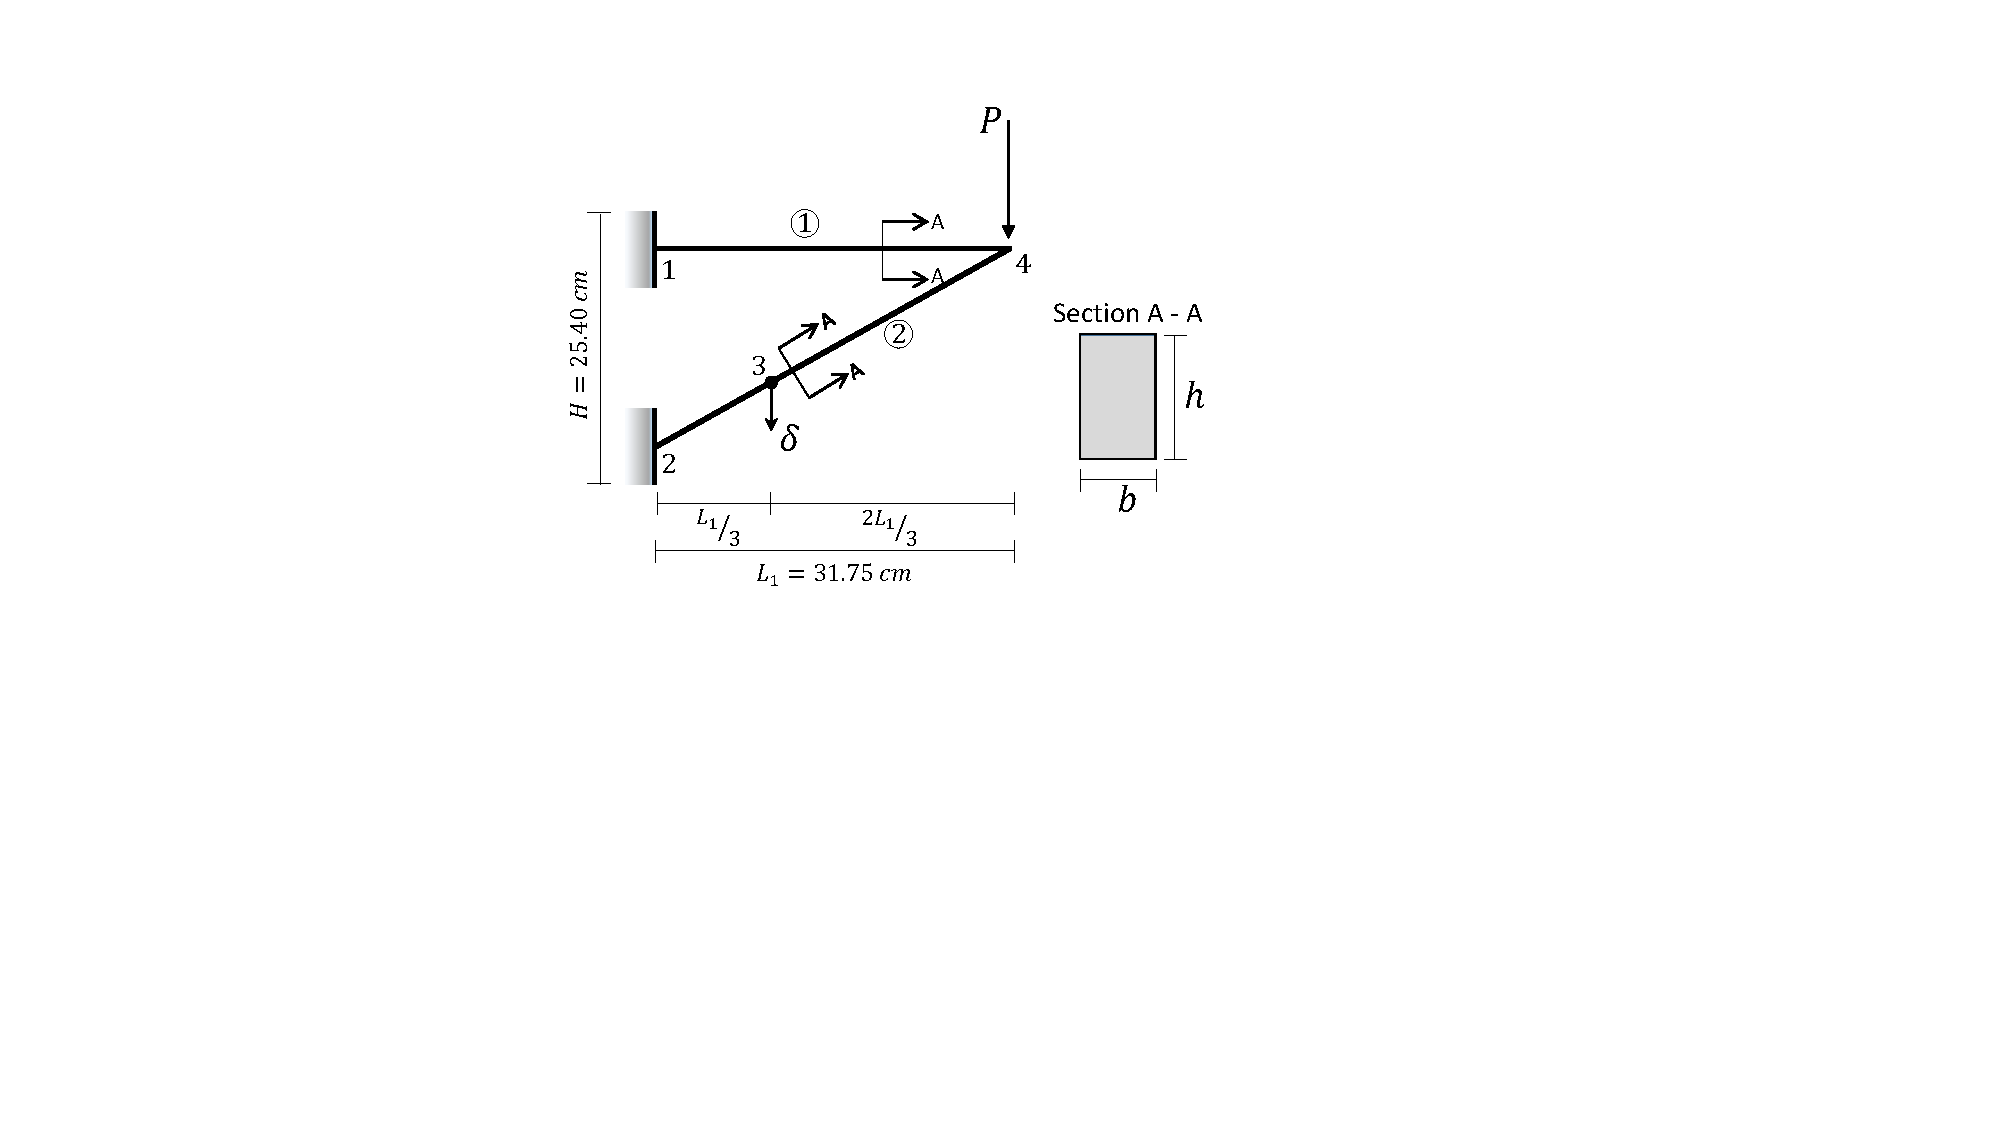
\includegraphics[width=0.45\textwidth]{FIG26_A_STRUCTURE}%
		\label{fig:FIG26_STRUCTURE}%
	}
	\subfloat[Load vs deflection at point B.]{%
		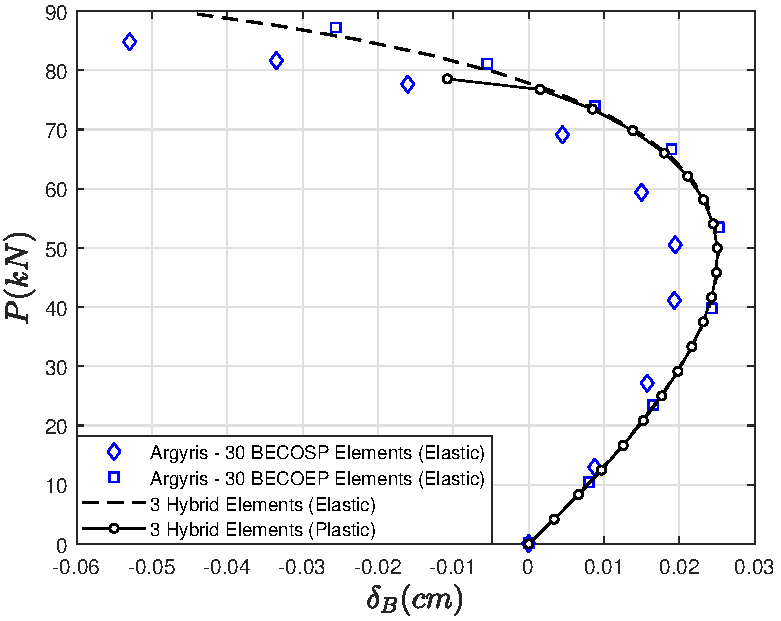
\includegraphics[width=0.45\textwidth]{FIG26_B_COMPARISON}%
		\label{fig:FIG26_COMPARISON}%
	}
	\caption{Geometry and loading of two-beam structure. Comparison of load vs 
		deflection curves for different cases.}
	\label{fig:FIG26}
\end{figure} 

\begin{figure}[b]
	\centering
	\subfloat[Elastic.]{%
		\hspace{-0.2cm}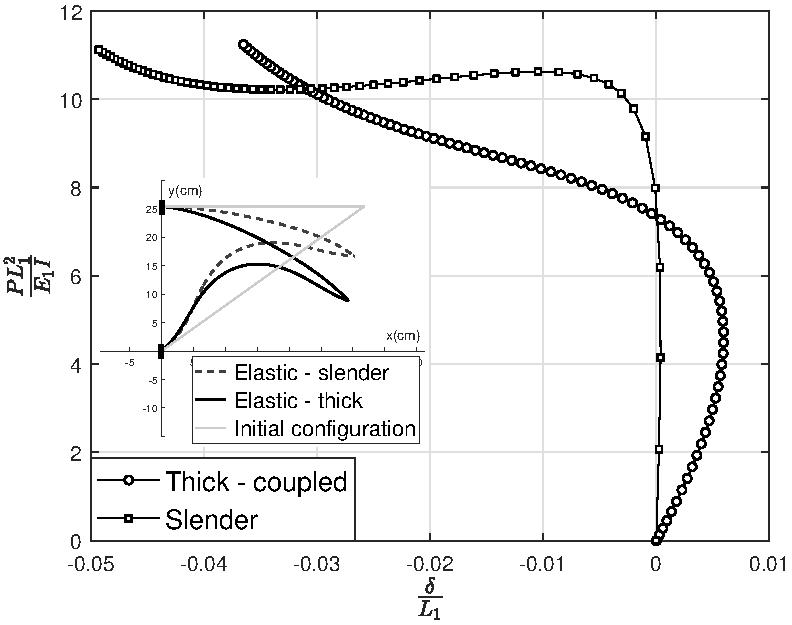
\includegraphics[width=0.45\textwidth]{FIG27_A_ELASTIC_COMPARISON}%
		\label{fig:FIG27_ELASTIC}%
	}
	\subfloat[Plastic.]{%
		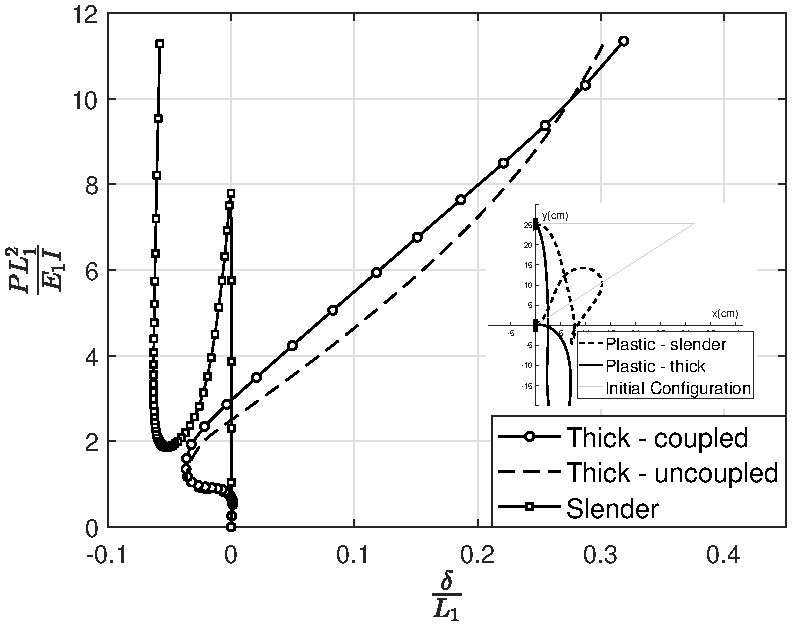
\includegraphics[width=0.45\textwidth]{FIG27_B_PLASTIC_COMPARISON}%
		\label{fig:FIG27_PLASTIC}%
	}
	\caption{Influence of slenderness and constitutive model on the response 
		for elastic and elastoplastic behavior.}
	\label{fig:FIG27}
\end{figure} 

 The full post-buckling elastoplastic equilibrium curve for 
the slender model is also provided for comparison. In 
Fig. \ref{fig:FIG27_ELASTIC} the post-buckling response of both slender and 
thick 
models are illustrated. In the former, both uniaxial and multiaxial 
constitutive models yield identical results, assuming an infinite yield stress.

As we reduce the slenderness, slight differences arise compared to a purely 
uniaxial behavior at the fiber. This is mainly due to the assumed strain 
distribution, which is user defined and not accounted in the purely flexural 
model.
\begin{figure}[b]
	\centering
	\subfloat[Step 15.]{%
		\hspace{-0.2cm}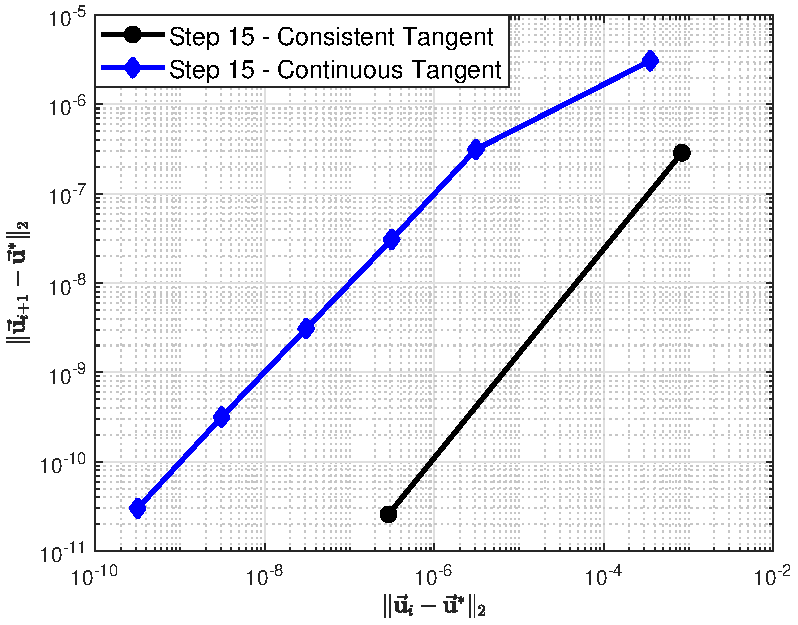
\includegraphics[width=0.45\textwidth]{STEP_15_RATES}%
		\label{fig:STEP15_RATES}%
	}
	\subfloat[Step 25.]{%
		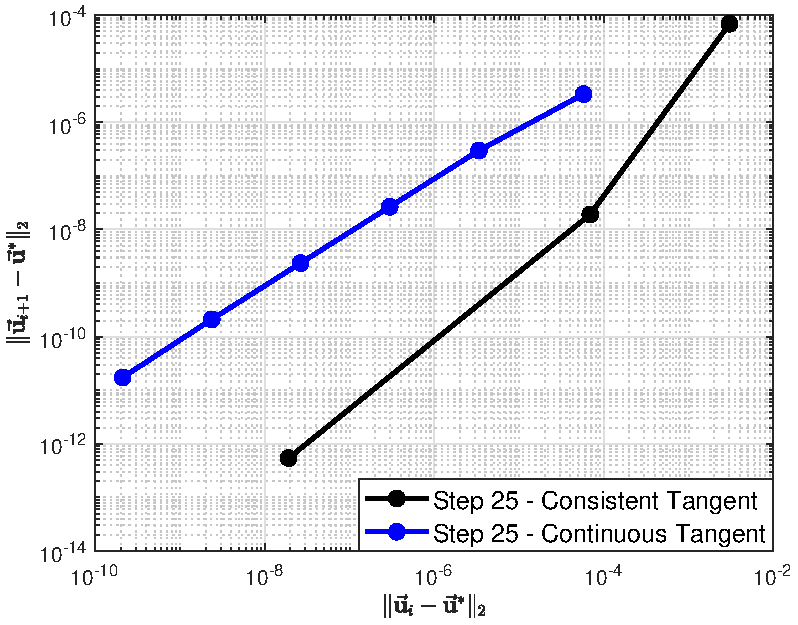
\includegraphics[width=0.45\textwidth]{STEP_25_RATES}%
		\label{fig:STEP25_RATES}%
	}
	\caption{Convergence rates for two representative steps when using the 
	consistent and continuous tangents at fibers.}
	\label{fig:RATES}
\end{figure} 

%% RESIDUAL NORM
\begin{table}
	\centering
	\begin{minipage}{0.8\linewidth}
		\caption{Convergence in residual norm during steps 5, 15, 25 35. 
			$\mathcal{\epsilon}_{tol}=10^{-10}$.}
		\label{table:TABLE8}
		\begin{tabular}{@ {}cllll@ {}}\toprule\toprule
			iters. & \hspace{0.8cm} 
			5 & \hspace{0.7cm} 15 & \hspace{0.7cm} 25 & \hspace{0.8cm} 35 \\
			\midrule
			1 & $1.000000\cdot 10^0$     & $1.000000\cdot 10^0$     & 
			$1.000000\cdot 10^0$     & $1.000000\cdot 10^0$ \\
			2 & $1.251499\cdot 10^{-2}$  & $1.988783\cdot 10^{-2}$ & 
			$1.737845\cdot 10^{-3}$  & $6.187773\cdot 10^{-2}$ \\
			3 & $2.132711\cdot 10^{-5}$  & $1.066255\cdot 10^{-5}$ & 
			$1.824164\cdot 10^{-6}$  & $4.214041\cdot 10^{-3}$ \\
			4 & $9.483080\cdot 10^{-10}$ & $4.882520\cdot 10^{-10}$ & 
			$2.229120\cdot 10^{-11}$ & $6.111545\cdot 10^{-5}$ \\
			5 & $5.150000\cdot 10^{-14}$ & $7.790000\cdot 10^{-13}$ & 
			$4.800000\cdot 10^{-14}$ & $1.218231\cdot 10^{-8}$  \\
			6 &  & &  & $7.110000\cdot 10^{-14}$\\
			\bottomrule\bottomrule[0.5pt] %\addlinespace[3pt]
		\end{tabular}
	\end{minipage}
\end{table}
\begin{table}%% ENERGY NORM 
	\centering
	\begin{minipage}{0.8\linewidth}
		\caption{Convergence in energy norm during steps 5, 15, 25, 35.%
			$\ \mathcal{\epsilon}_{tol}=10^{-10}$.}
		\label{table:TABLE9}
		\begin{tabular}{@ {}cllll@ {}}\toprule\toprule
			iters.  & 
			\hspace{0.8cm} 5 & \hspace{0.7cm} 15 & \hspace{0.7cm} 25 & 
			\hspace{0.8cm} 35 \\
			\midrule
			1 & $1.000000\cdot 10^0$    &  $1.000000\cdot 10^0$  & 
			$1.000000\cdot 10^0$ & $1.000000\cdot 10^0$ \\
			2 & $3.050574\cdot 10^{-4}$  &  $1.065944\cdot 10^{-4}$ & 
			$2.618542\cdot 10^{-2}$ & $1.188951\cdot 10^{-2}$ \\
			3 & $2.235712\cdot 10^{-5}$  &  $5.373434\cdot 10^{-5}$ & 
			$4.974768\cdot 10^{-5}$ & $1.495507\cdot 10^{-4}$ \\
			4 & $1.532842\cdot 10^{-8}$  &  $2.585263\cdot 10^{-9}$ & 
			$1.551550\cdot 10^{-7}$ & $1.706384\cdot 10^{-5}$ \\
			5 & $6.283000\cdot 10^{-12}$ &  $1.962000\cdot 10^{-12}$ & 
			$1.687900\cdot 10^{-11}$ & $3.948037\cdot 10^{-7}$  \\
			7 &  & &  & $5.157400\cdot 10^{-11}$ \\
			\bottomrule\bottomrule[0.5pt] %\addlinespace[3pt]
		\end{tabular}
	\end{minipage}
\end{table}

\clearpage

%%%%%%%%%%%%%%%%%%%%  EXAMPLE 5 %%%%%%%%%%%%%%%%%%%%%%%%%%%%%%%%
\subsection{Three Story Frame With Shear Links}

The three-story four-bay steel frame, first analyzed in \cite{Amir2022}, is 
shown in Fig. \ref{fig:FIG28_STRUCTURE}, where the diagonal braces are ignored. 
Gravity loads are 
derived from the material and geometric properties of the elements and, for 
simplicity, are assumed to be acting on frame joints only. The values for each 
joint gravity load are shown in Table \ref{table:TABLE10}. 

\begin{table}[h]
	\centering
	\begin{minipage}{0.7\linewidth}
		\caption{Vertical gravity loads at nodes.}
		\begin{tabular}{cccccccccc}
			\toprule\toprule
			Nodes                         & 2,18 & 3,19 & 4,20& 6,14 & 7,15 & 
			8,16 & 10 & 11 & 12 \\
			\midrule
			$\downarrow P_i \text{(kN)}$  & 240  & 220  & 145 & 340 & 300 & 190 
			& 255 & 215 & 120 \\
			\bottomrule\bottomrule
			\label{table:TABLE10}
		\end{tabular}
	\end{minipage}
\end{table}

A static pushover analysis is then conducted with respect to the 
superimposed horizontal loads on nodes 2,3, 
and 4. All members have 
the same yield stress and Young's modulus: $\sigma_y = 290$ MPa, $E = 210$ GPa, 
and the Poisson's ratio is set to $\nu= 0.3$. Both material and geometric 
nonlinearity options are activated for the 
analysis and perfect plasticity is assumed. In Fig. \ref{fig:FIG28_EQPATHS} we 
compare the results we get using the hybrid \acrshort{nlp} element with the 
nonlinear flexibility element in 
OpenSees\cite{OpenSees}. In OpenSees we used two different modelling approaches 
with regards to cross-section constitutive behavior: 1) a purely flexural fiber 
section and 2) a section aggregator object, whereby a uniaxial shear 
force-strain law is overloaded on an existing fiber section. In the latter 
approach, the flexural and shear effects remain uncoupled. For the analyses 
using the proposed element, we again adopted 2 different approaches. In the 
first approach we assumed an uncoupled section constitutive law, whereby 
axial-flexural effects are determined by integrating the relevant equations 
over the section fibers while the shear effects are assumed concentrated in the 
centerline. The underlying assumption in this approach is that the shear 
strains are uniform. For the second approach we assumed full coupling at the 
section fibers utilizing the J2 constitutive law and computationally solving 
the stress update problem using the return mapping algorithm proposed in this 
chapter. As can be seen 
from \ref{fig:FIG28_EQPATHS}, the results we get with aggregator sections in 
OpenSees are, expectably, identical with the uncoupled constitutive model when 
using the \acrshort{nlp} element. Both predict a higher  
collapse load than the fully coupled \acrshort{nlp}, which is also an expected 
result. The purely flexural model in OpenSees gives an even slightly higher 
collapse load than the uncoupled models. It is clear that, in the presence of 
shearing components, such as the effective shear wall in this example, a purely 
flexural model will result in non-conservative estimates even in simple 
push-over analyses.  

To 
achieve convergent results, the analyses with OpenSees required 90 elements 
with six Gauss-Lobatto points per element for the section aggregator model and 
ten points for the purely flexural model. Each member besides the shear 
links was discretized into 4 nonlinear beam-column elements. In contrast, for 
the analyses using the element proposed in Chapter 2 only one hybrid element 
per 
member was required, resulting in 27 elements in total, and five Gauss-Lobatto 
quadrature points per 
element. Both models account for second order effects under the presence of 
gravity loads.

\begin{figure}
	\centering
	\subfloat[Frame structure.]{%
		\hspace{-0.2cm}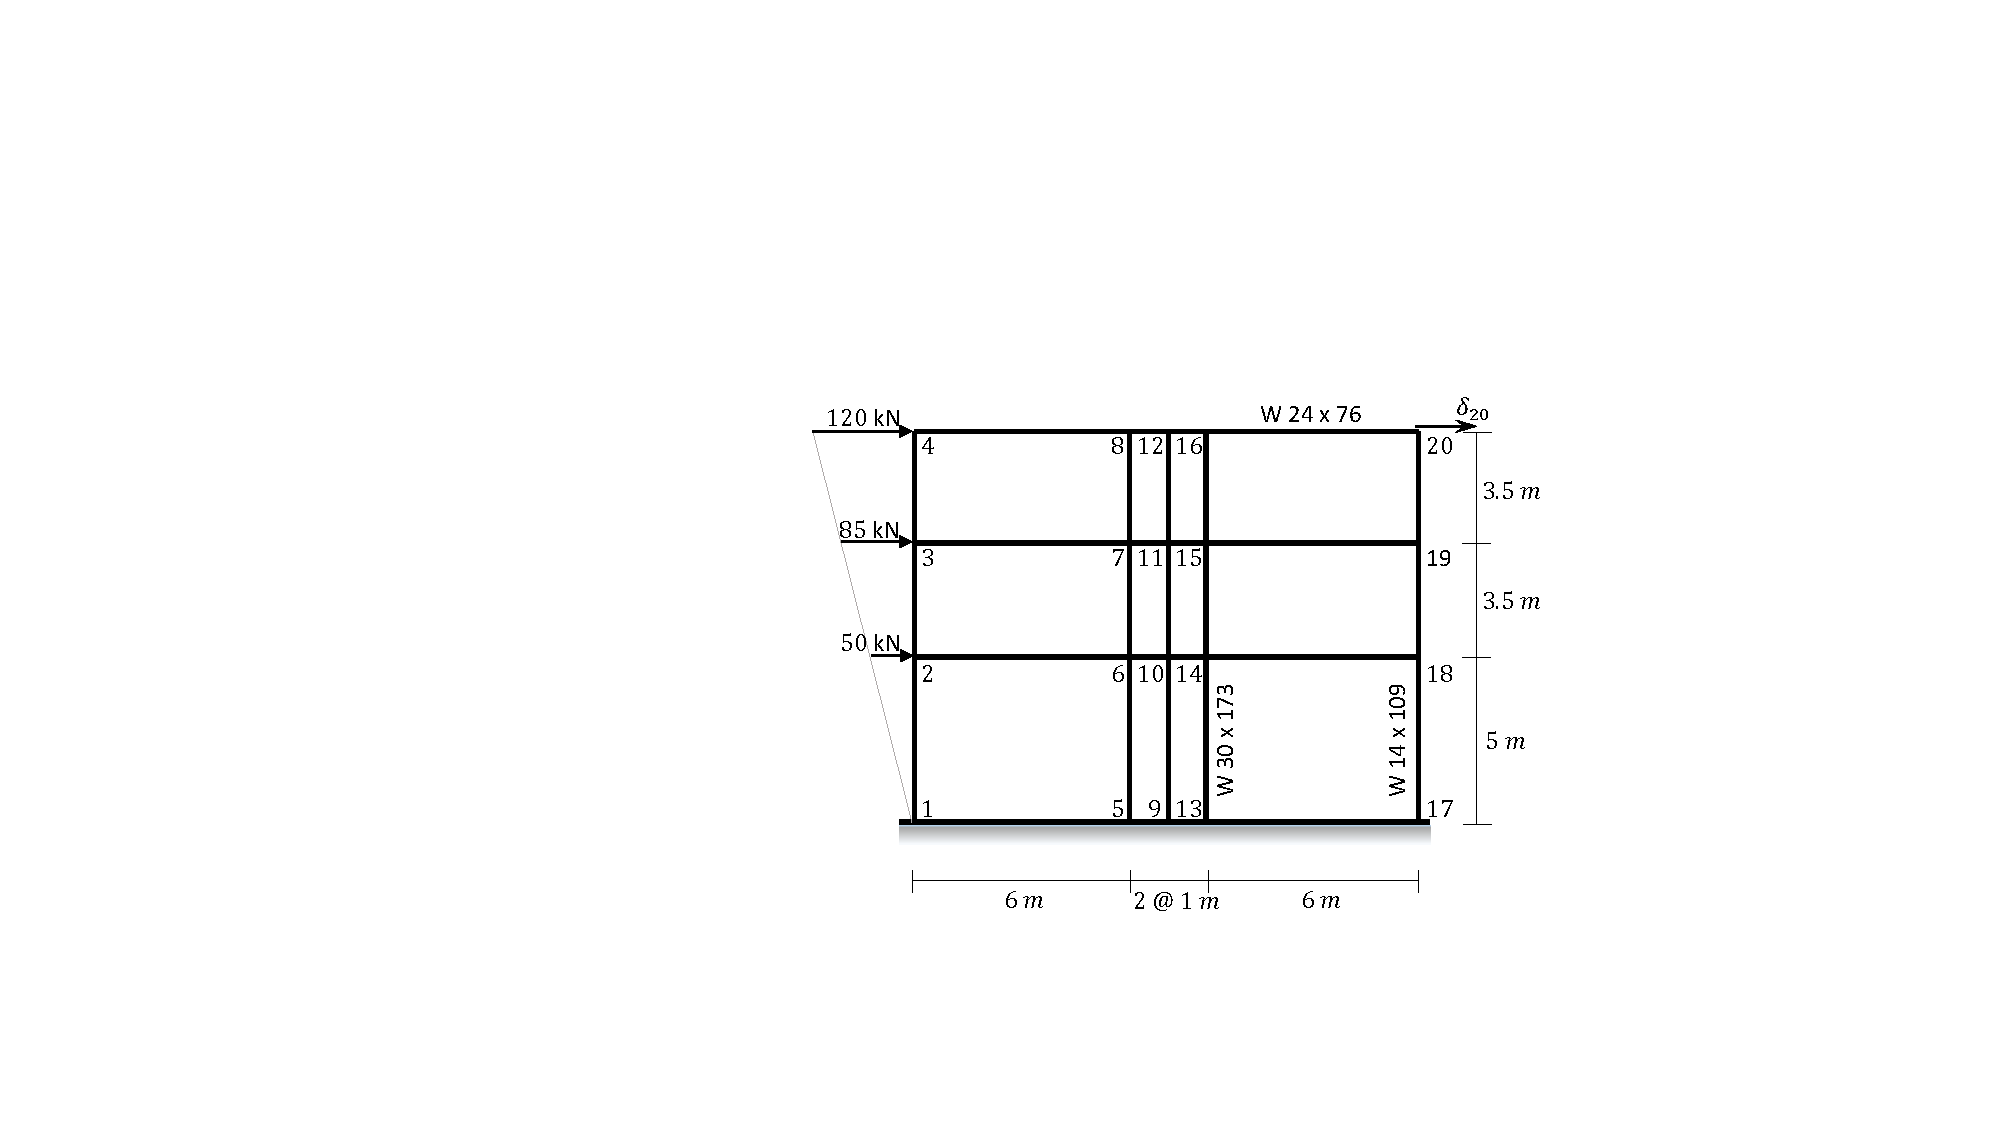
\includegraphics[width=0.45\textwidth]{FIG28_STRUCTURE}%
		\label{fig:FIG28_STRUCTURE}%
	}
	\subfloat[Equilibrium paths.]{%
		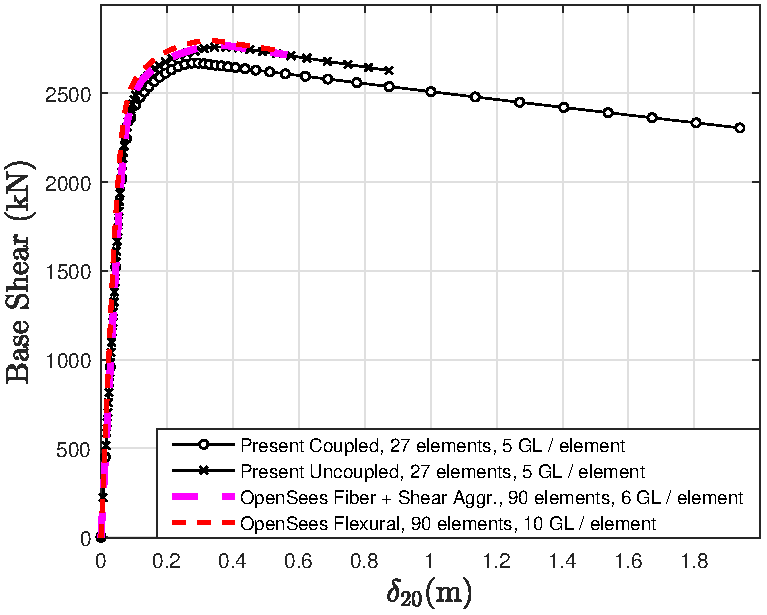
\includegraphics[width=0.45\textwidth]{FIG28_EQPATHS}%
		\label{fig:FIG28_EQPATHS}%
	}
	\caption{Geometry of the steel frame and \ref{fig:FIG28_EQPATHS} response 
		curves for three different models.}
	\label{fig:FIG28}
\end{figure}

%the results we get for 3 
%different modelling 
%options regarding the constitutive law at the fiber level. Both the purely 
%flexural model and the uncoupled elastoplastic model, whereby shear and axial 
%states on fibers are uniaxial and do not interract, yield the same response 
%curve and collapse load. In contrast, the coupled multiaxial model predicts, 
%again, a lower plastic capacity load. 


\section{Summary}

In this chapter a return mapping algorithm for planar, shear 
flexible beam finite elements was presented that fully accounts for 
shear-axial-flexure 
interaction. The proposed formulation is particularly suited for 
flexibility-based or 
hybrid-type elements, which tend to rely more on higher order quadrature rules. 
Focusing our attention in the von Mises yield criterion with both linear 
kinematic and 
isotropic hardening, we have shown that the proposed model is much faster in 
terms of computational cost than 
conventional stress update procedures typically implemented in beam models. In 
addition, we derived the material tangent modulus consistent with the fully 
implicit Euler scheme used for the integration of rate constitutive equations, 
as well as the general form of the consistent section tangent stiffness. It was 
seen that 
the latter depends on the return mapping scheme and the assumption on shear 
strain 
distribution on the cross-section. Use of consistent tangents is crucial in the 
numerical treatment of such problems because they restore the quadratic rates 
of 
converge for the global Newton method. Lastly, the accuracy and efficacy of the 
proposed 
framework was demonstrated in a number of numerical problems, presented in the 
last section. 